\documentclass{article}

\usepackage{ijcai11}

\usepackage{times}
\usepackage{amsmath,amsfonts,amssymb}
\usepackage{hhline}
\usepackage[dvipsnames,usenames]{xcolor}
\usepackage{pifont} \usepackage{subfig}
\usepackage{tikz}
\usetikzlibrary{patterns}
\usetikzlibrary{calc}
\usetikzlibrary{decorations.pathmorphing}
\graphicspath{{5-1-Graphics/}{/}}
\usepgfmodule{plot}
\usepackage{url}

\newtheorem{theorem}{Theorem}
\newtheorem{lemma}[theorem]{Lemma}
\newtheorem{corollary}[theorem]{Corollary}



\newcommand{\nb}[1]{\marginpar{\scriptsize\raggedright\textcolor{red}{#1}}}

\newcommand{\ic}{c^\circ}
\newcommand{\NP}{\textsc{NP}}
\newcommand{\PSpace}{\textsc{PSpace}}
\newcommand{\ExpTime}{\textsc{ExpTime}}
\newcommand{\Sat}{\textit{Sat}}

\newcommand{\cB}{\mathcal{B}}\newcommand{\cBC}{\mathcal{C}}\newcommand{\cBc}{\ensuremath{\mathcal{B}c}}
\newcommand{\cBci}{\ensuremath{\mathcal{B}c^\circ}}
\newcommand{\RCCE}{\ensuremath{\mathcal{RCC}8}}\newcommand{\RCCF}{\ensuremath{\mathcal{RCC}5}}\newcommand{\BRCCE}{\ensuremath{\mathcal{BRCC}8}}\newcommand{\RCCEc}{\ensuremath{\RCCE{}c}}\newcommand{\RCCEci}{\ensuremath{\RCCE{}c^\circ}}\newcommand{\cBCc}{\ensuremath{\mathcal{C}c}}\newcommand{\cBCci}{\ensuremath{\mathcal{C}c^\circ}}

\newcommand{\R}{\mathbb{R}}
\newcommand{\RC}{{\sf RC}}
\newcommand{\RCP}{{\sf RCP}}

\newcommand{\fw}{\mathsf{w}}
\newcommand{\fW}{\mathbf{w}}

\newcommand{\cL}{\mathcal{L}}

\newcommand{\ti}[2][]{{#2}^{\circ_{#1}}}
\newcommand{\tc}[2][]{{#2}^{-_{#1}}}

\newcommand{\set}[1]{\{#1\}}
\newcommand{\tseq}[1]{\mathfrak{#1}}
\newcommand{\intermediate}[1]{\dot{#1}}
\newcommand{\inner}[1]{\ddot{#1}}
\newcommand{\stack}{\mathsf{stack}}
\newcommand{\stacki}{\ti{\mathsf{stack}}}
\newcommand{\frameFla}{\mathsf{frame}}
\newcommand{\frameFlai}{\ti{\mathsf{frame}}}
\newcommand{\md}[2][] {{\lfloor#2\rfloor_{#1}}}

\newcommand{\qedsymbol}{\ding{113}}
\newenvironment{proof}{\par\noindent\textbf{Proof.}}{\mbox{}\hfill\qedsymbol\par\bigskip}
\newenvironment{swetheorem}[1]{\par\medskip\noindent\textbf{#1.}\hspace*{0.5em}\em}{\par\smallskip}


\renewcommand{\phi}{\varphi}



\title{On the Decidability of Connectedness Constraints in 2D and 3D Euclidean Spaces}
\author{Roman Kontchakov\!, Yavor Nenov\!, Ian Pratt-Hartmann and Michael Zakharyaschev\\
{\parbox[t]{60mm}{\centering Department of Computer Science and Information Systems\\ Birkbeck College London, U.K.}}\hspace*{3em}
\parbox[t]{60mm}{\centering School of Computer Science\\ University of Manchester, U.K.}}

\begin{document}

\maketitle

\begin{abstract}
We investigate (quantifier-free) spatial constraint languages with
equality, contact and connectedness predicates, as well as Boolean
operations on regions, interpreted over low-dimensional Euclidean
spaces. We show that the complexity of reasoning varies dramatically
depending on the dimension of the space and on the type of regions
considered. For example, the logic with the interior-connectedness
predicate (and without contact) is undecidable over polygons or
regular closed sets in , \ExpTime-complete over polyhedra in
, and \NP-complete over regular closed sets in .
\end{abstract}




\section{Introduction}\label{sec:intro}

A central task in Qualitative Spatial Reasoning is that of determining
whether some described spatial configuration is geometrically
realizable in 2D or 3D Euclidean space. Typically, such a description
is given using a spatial logic---a formal language whose variables
range over (typed) geometrical entities, and whose non-logical
primitives represent geometrical relations and operations involving
those entities. Where the geometrical primitives of the language are
purely topological in character, we speak of a \emph{topological
  logic}; and where the logical syntax is confined to that of
propositional calculus, we speak of a \emph{topological constraint
  language}.

Topological constraint languages have been intensively studied in
Artificial Intelligence over the last two decades.  The best-known of
these, \RCCE{} and \RCCF, employ variables ranging over regular closed
sets in topological spaces, and a collection of eight (respectively,
five) binary predicates standing for some basic topological relations
between these
sets~\cite{ijcai:Egenhofer&Franzosa91,ijcai:Randelletal92,ijcai:Bennett94,ijcai:Renz&Nebel98}. An
important extension of \RCCE, known as \BRCCE{}, additionally features
standard Boolean operations on regular closed
sets~\cite{ijcai:Wolter&Z00ecai}.

A remarkable characteristic of these languages is their
\emph{in}sensitivity to the underlying interpretation.  To show that an
\RCCE-formula is satisfiable in -dimensional Euclidean space, it
suffices to demonstrate its satisfiability in {\em any} topological
space \cite{ijcai:Renz98}; for \BRCCE-formulas, satisfiability in
\emph{any connected} space is enough. This inexpressiveness yields
(relatively) low computational complexity: satisfiability
of~\BRCCE-, \RCCE- and \RCCF-formulas over arbitrary topological
spaces is \NP-complete; satisfiability of~\BRCCE{}-formulas over
connected spaces is \PSpace-complete.

However, satisfiability of spatial constraints by {\em arbitrary}
regular closed sets by no means guarantees realizability by
practically meaningful geometrical objects, where {\em connectedness}
of regions is typically a minimal
requirement~\cite{Borgo96,ijcai:Cohn&Renz08}.  (A connected region is
one which consists of a `single piece.')  It is easy to write
constraints in  that are satisfiable by connected regular
closed sets over arbitrary topological spaces but not over ; in
 we can even write formulas satisfiable by connected regular
closed sets over arbitrary spaces but not over  for any .
Worse still: there exist very simple collections of spatial
constraints (involving connectedness) that are satisfiable in the
Euclidean plane, but only by `pathological' sets that cannot plausibly
represent the regions occupied by physical objects~\cite{ijcai:HSL2}.
Unfortunately, little is known about the complexity of topological
constraint satisfaction by non-pathological objects in low-dimensional
Euclidean spaces. One landmark result~\cite{ijcai:iscloes:sss03} in
this area shows that satisfiability of \RCCE-formulas by
\emph{disc-homeomorphs} in  is still \NP-complete, though the
decision procedure is vastly more intricate than in the general
case. In this paper, we investigate the computational properties of
more general and flexible spatial logics with connectedness
constraints interpreted over  and .

We consider two `base' topological
constraint languages.  The language  features  as its
only predicate, but has function symbols , ,  denoting
the standard operations of fusion, complement and taking common parts
defined for regular closed sets, as well as the constants  and 
for the entire space and the empty set. Our second base language,
, additionally features a binary predicate, , denoting the
`contact' relation (two sets are in {\em contact} if they share at
least one point).  The language  is a notational variant
of~\BRCCE{} (and thus an extension of \RCCE), while  is the
analogous extension of \RCCF{}. We add to  and  one of
two new unary predicates: , representing the property of
connectedness, and , representing the (stronger) property of
having a connected \emph{interior}. We denote the resulting languages
by , \!,  and \!. We are interested 
in interpretations over ({\em i}) the regular closed sets of 
and , and ({\em ii}) the regular closed \emph{polyhedral} sets
of  and .  (A set is polyhedral if it can be defined by
finitely many bounding hyperplanes.) By restricting interpretations to
polyhedra we rule out satisfaction by pathological sets and use the
same `data structure' as in GISs.

When interpreted over {\em arbitrary} topological spaces, the
complexity of reasoning with these languages is known: satisfiability
of -formulas is \NP-complete, while for the other three
languages, it is \ExpTime-complete.  Likewise, the 1D Euclidean case
is completely solved.  For the spaces  (), however,
most problems are still open.  All four languages contain
formulas satisfiable by regular closed sets in , but not by
regular closed polygons; in , the analogous result is known
only for  and . The satisfiability problem for \cBc{},
\cBCc{} and \cBCci{} is \ExpTime-hard (in both polyhedral and
unrestricted cases) for  (); however, the only known
upper bound is that satisfiability of -formulas by
polyhedra in  () is \ExpTime-complete.
(See~\cite{ijcai:kphz10} for a summary.)

This paper settles most of these open problems, revealing considerable
differences between the computational properties of constraint
languages with connectedness predicates when interpreted over 
and over abstract topological spaces.  Sec.~\ref{sec:sensitivity}
shows that , ,  and  are all sensitive to
restriction to polyhedra in  (). Sec.~\ref{sec:undecidability} establishes an unexpected result:
all these languages are \emph{undecidable} in 2D, both in the
polyhedral and unrestricted cases (\cite{Dornheim} proves
undecidability of the \emph{first-order} versions of these
languages). Sec.~\ref{sec:3d} resolves the open issue of the
complexity of  over regular closed sets (not just polyhedra) in
 by establishing an NP upper bound.  Thus, Qualitative Spatial
Reasoning in Euclidean spaces proves much more challenging if
connectedness of regions is to be taken into account.  We discuss the
obtained results in the context of spatial reasoning in
Sec.~\ref{conclusion}.  Omitted proofs can be found in the appendix. 






\section{Constraint Languages with Connectedness}\label{sec:preliminaries}

Let  be a topological space. We denote the closure of any  by , its interior by  and its boundary by
. We call  {\em regular closed}
if , and denote by  the set of regular closed
subsets of . Where  is clear from context, we refer to elements
of  as {\em regions}.  forms a Boolean algebra under
the operations ,  and . We write  for ; thus
 iff .  A subset  is
\emph{connected} if it cannot be decomposed into two disjoint,
non-empty sets closed in the subspace topology;  is
\emph{interior-connected} if  is connected.

Any -dimensional hyperplane in , , bounds two
elements of  called \emph{half-spaces}. We denote by
 the Boolean subalgebra of  generated by the
half-spaces, and call the elements of  (regular closed)
\emph{polyhedra}. If , we speak of (regular closed)
\emph{polygons}. Polyhedra may be regarded as `well-behaved' or, in
topologists' parlance, `\emph{tame}.'  In particular, every polyhedron
has finitely many connected components, a property which is not true
of regular closed sets in general.

The topological constraint languages considered here all employ a
countably infinite collection of variables  The
language  features binary predicates  and , together with
the individual constants ,  and the function symbols ,
, . The \emph{terms}  and \emph{formulas}  of
 are given by:

The language  is defined analogously, but without the predicate
. If  for some topological space , an
\emph{interpretation over}  is a function 
mapping variables  to elements . We extend
 to terms  by setting , , , etc. We write
 iff , and  iff
.  We
read  as ` \emph{contacts} .'  The
relation  is extended to non-atomic formulas in the obvious
way. A formula  is \emph{satisfiable over}  if 
 for some interpretation  over . 

Turning to languages with connectedness predicates, we define 
and  to be extensions of  and  with the unary
predicate . We set  iff
 is connected in the topological space under
consideration. Similarly, we define  and  to be
extensions of  and  with the predicate , setting
 iff  is connected.  is the set of -formulas
satisfiable over , where 
is one of , ,  or  (the
topological space is implicit in this notation, but will always be
clear from context). We shall be concerned with , where
 is  or  for .

To illustrate, consider the -formulas 
given by

One can show that  is satisfiable over , , but not over , as no three intervals with non-empty,
disjoint interiors can be in pairwise contact. Also,  is
satisfiable over , for , but not over
, as the graph  is non-planar.  Thus,  is
sensitive to the dimension of the space.
Or again, consider the -formula 

One can show that~\eqref{eq:wiggly} is satisfiable over ,
for any  (see, e.g., Fig.~\ref{fig:wiggly}), but not over
. Thus  is sensitive to tameness in Euclidean
spaces.
\begin{figure}[ht]
\begin{center}
\resizebox{3.1cm}{!}{\begin{picture}(0,0)\includegraphics{wiggly.pstex}\end{picture}\setlength{\unitlength}{1579sp}\begingroup\makeatletter\ifx\SetFigFont\undefined \gdef\SetFigFont#1#2#3#4#5{\reset@font\fontsize{#1}{#2pt}\fontfamily{#3}\fontseries{#4}\fontshape{#5}\selectfont}\fi\endgroup \begin{picture}(8355,5918)(2119,-6436)
\put(2701,-2086){\makebox(0,0)[lb]{\smash{{\SetFigFont{24}{9.6}{\rmdefault}{\mddefault}{\updefault}{\color[rgb]{0,0,0}}}}}}
\put(9751,-5086){\makebox(0,0)[lb]{\smash{{\SetFigFont{24}{9.6}{\rmdefault}{\mddefault}{\updefault}{\color[rgb]{0,0,0}}}}}}
\put(9601,-1636){\makebox(0,0)[lb]{\smash{{\SetFigFont{24}{9.6}{\rmdefault}{\mddefault}{\updefault}{\color[rgb]{0,0,0}}}}}}
\end{picture} }
\end{center}\vspace*{-3mm}
\caption{Three regions in  satisfying \eqref{eq:wiggly}.}
\label{fig:wiggly}
\end{figure}
It is known~\cite{ijcai:kphz10} that, for the Euclidean {\em plane},
the same is true of  and : there is a -formula
satisfiable over , but not over . (The 
example required to show this is far more complicated than the
\cBci-formula~\eqref{eq:wiggly}.)  In the next section, we prove that
any of ,  and  contains formulas satisfiable
over , for every , but only by regions with
infinitely many components. Thus, all four of our languages are
sensitive to tameness in all dimensions greater than one.





\section{Regions with Infinitely Many Components}\label{sec:sensitivity}

Fix  and let  be regions partitioning :

We construct formulas forcing the  to have infinitely many
connected components. To this end we require non-empty regions 
contained in , and a non-empty region :

The configuration of regions we have in mind is depicted in
Fig.~\ref{fig:InfCmpSat}, where components of the  are arranged
like the layers of an onion. The `innermost' component of  is
surrounded by a component of , which in turn is surrounded by a
component of , and so on. The region  passes through every
layer, but avoids the . To enforce a configuration of this sort,
we need the following three formulas, for :

where . Formulas~\eqref{eq:InfContact} and
\eqref{notC} ensure that each component of  is in contact with
, while \eqref{eq:InfNTriv1} ensures that no component of
 can touch any component of .
\begin{figure}[h]
\begin{center}
\begin{tikzpicture}
\small
	\coordinate (Px) at (-3.7,0);
	\coordinate (Qx) at (1.2,0);
	\coordinate (Py) at (0,1);
	\coordinate (Pby) at (0,.5);
	\foreach \i/\a/\b in {1/40/20,0/25/10,3/40/20,2/25/10,1/40/20,0/25/10}
	{
		\draw[thick,fill=black!\b] () rectangle ();
		\draw[thin,fill=black!\b] () rectangle ();
		\draw[thick] () rectangle ();
		\node at () {};
		\node at () {};
		\coordinate (Px) at ();
		\coordinate (Py) at ();
		\coordinate (Pby) at ();
		\coordinate (Qx) at ();
	}
	\draw (4.3,0.7)--(.5,0.25)--(.5,0.2)--(4.3,0.2);
	\node at (4.1,.4) {};
	\node at (4.1,0) {};
\end{tikzpicture}		
\end{center}
\vspace*{-2mm}
\caption{Regions satisfying .}\label{fig:InfCmpSat}	
\end{figure}

Denote by  the conjunction of the above
constraints. Fig.~\ref{fig:InfCmpSat} shows how  can be
satisfied over . By cylindrification, it is also satisfiable
over any , for .

The arguments of this section are based on the following
property of regular closed subsets of Euclidean spaces:
\begin{lemma}\label{lma:ourNewman}
If  is connected, then every component of  
has a connected boundary.
\end{lemma}

The proof of this lemma, which follows from a result
in~\cite{ijcai:Newman64}, can be found in Appendix~\ref{sec:sensitivityA}. 
The result fails for other familiar spaces such as the torus.
\begin{theorem}\label{theo:inftyCc}
There is a -formula 
satisfiable over , , but not by regions with finitely many components.
\end{theorem}
\begin{proof}
Let  be as above.
To simplify the presentation, we ignore the difference between variables
and the regions they stand for, writing, for example,  instead of
.  We construct a sequence of disjoint components
 of  and open sets  connecting  to
 (Fig.~\ref{fig:InfCmpConstr}). By the first conjunct
of~\eqref{eq:basic-regions}, let  be a component of 
containing points in . Suppose  has been constructed.
By~\eqref{eq:InfContact} and~\eqref{notC},  is in contact with
. Using~\eqref{eq:InfNTriv1} and the fact that
 is locally connected, one can find a
component  of  which has points in ,
and a connected open set  such that  and  are non-empty, but  is empty.
\begin{figure}[h]
\begin{center}
\begin{tikzpicture}
	\newcommand{\iterateboxes}[3][]
	{
		\coordinate (Plx) at (0,0);
		\coordinate (Prx) at (7.5,0);
		\coordinate (Py) at (0,1);
		#1
		\foreach \x/\y in {3/2,2/1,1/0}
		{
			#2
			
			\coordinate (Plx) at ();
			\coordinate (Prx) at ();
			\coordinate (Py) at ();
		}
		#3
	}
	\small
	\iterateboxes
	[\node at () {};]
	{
		\draw[draw=black,fill=gray!30] () rectangle ();
		\draw[draw=black,thick,fill=gray!0] () rectangle ();
\node at () {};
	}
	{
		\draw[draw=black,fill=gray!30] () rectangle ();
		\node at () {};
	}
	\iterateboxes
	{
		\filldraw () coordinate(P);
		\filldraw () coordinate(Q);
		\draw () ellipse (.5 and 0.2);
		\node at () {};
	}{}
\end{tikzpicture}
\end{center}
\vspace*{-2mm}
\caption{The sequence  generated by .
( and  are the `holes' of  containing  and .)
}
\label{fig:InfCmpConstr}
\end{figure}


To see that the  are distinct, let  and  be the
components of  containing  and ,
respectively. It suffices to show .
Note that the connected set  must intersect .
Evidently, .
Also, ; hence,
by~\eqref{eq:InfPart1} and~\eqref{eq:InfNTriv1}, .  By Lemma~\ref{lma:ourNewman},
 is connected, and therefore, by~\eqref{eq:InfNTriv1},
is entirely contained either in  or in
. Since  and
, we have , so . Similarly,
.  By~\eqref{eq:InfNTriv1}, then,
, and since 
and  are components of the same set, they are
disjoint. Hence, , and since
, also . So,  lies in the interior of
a component of , and since , that component must be .
\end{proof}

\vspace*{-2mm}

Now we show how the -formula  can be transformed
to - and -formulas with similar properties.  Note first
that all occurrences of  in  have positive polarity.
Let  be the result of replacing them with the
predicate . In Fig.~\ref{fig:InfCmpSat}, the connected regions
mentioned in~\eqref{eq:InfContact} are in fact interior-connected;
hence  is satisfiable over . Since
interior-connectedness implies connectedness, 
entails , and we obtain:
\begin{corollary}\label{cor:inftyCci}
There is a -formula 
satisfiable over , , but not by regions with finitely many components.
\end{corollary}

To construct a -formula, we observe
that all occurrences of  in  are negative. We eliminate
these using the predicate . Consider, for example, the formula
) in~\eqref{notC}.
By inspection of Fig.~\ref{fig:InfCmpSat},
one can find regions ,  satisfying

On the other hand, \eqref{eq:contactTrick} entails . By
treating all other non-contact relations similarly, we obtain a
-formula  that is satisfiable over , and
that entails . Thus:
\begin{corollary}\label{cor:inftyBc}
There is a -formula satisfiable over , ,
but not by regions with finitely many components.
\end{corollary}

Obtaining a  analogue is complicated by the fact that we must
enforce non-contact constraints using  (rather than ). In the
Euclidean plane, this can be done using \emph{planarity constraints};
see Appendix~\ref{sec:sensitivityA}.
\begin{theorem}\label{theo:inftyBci}
There is a -formula satisfiable over , but not by
regions with finitely many components.
\end{theorem}

Theorem~\ref{theo:inftyCc} and Corollary~\ref{cor:inftyBc} entail that, if
 is  or , then  for .  Theorem~\ref{theo:inftyBci}
fails for  with  (Sec.~\ref{sec:3d}).  However, we
know from~\eqref{eq:wiggly} that  for all . Theorem~\ref{theo:inftyCc}
fails in the 1D case; moreover, 
only in the case  or ~\cite{ijcai:kphz10}.





\section{Undecidability in the Plane}\label{sec:undecidability}

Let  be any of , ,  or . In this
section, we show, via a reduction of the {\em Post correspondence
  problem} (PCP), that  is r.e.-hard, and
 is r.e.-complete. An {\em instance} of the PCP
is a quadruple  where  and  are
finite alphabets, and each  is a word morphism from  to
. We may assume that  and  is non-empty
for any . The instance  is {\em positive} if there
exists a non-empty  such that . The set
of positive PCP-instances is known to be r.e.-complete. The reduction
can only be given in outline here: full details are given in 
Appendix~\ref{sec:UndecidabilityB}.



To deal with arbitrary regular closed subsets of , we use
the technique of `wrapping' a region inside two bigger ones. Let us
say that a \emph{3-region} is a triple  of elements of  such that
, where 
abbreviates . It helps to think of  as consisting of a kernel,
, encased in two protective layers of shell. As a simple
example, consider the sequence of 3-regions  depicted in Fig.~\ref{fig:stack}, where the inner-most
regions form a sequence of externally touching polygons.
\begin{figure}[h]
\begin{center}
\begin{tikzpicture}[	s0/.style={fill=Gray!40,fill opacity=0.5},			s1/.style={dashed,fill=Gray!20,fill opacity=0.3},			s2/.style={dotted,fill=white,fill opacity=0}] 		

	\newcount\mod
	\newcount\jj
	
	\coordinate (H0) at (2,0); \coordinate (V0) at (0,0.8); \coordinate (H1) at (2,0); \coordinate (V1) at (0,.4); 

	\coordinate (HW) at (.4,0); \coordinate (VW) at (0,.2); \coordinate (P) at (0,0);
	
	\foreach \j in {2,1,0}
	{
	   \foreach \i in {1,2,3}{			
		    \pgfmathsetcount{\mod}{mod(\i,2)}
			\coordinate (H) at (); \coordinate (V) at (); 

			\filldraw[s\j] ()
				--++()
				--++()
				--++()
				--++()
				--++()
				--++()
				--++()
				--++();			
			\ifnum \j=0 \node at () {\small }; \fi
			\ifnum \j=1 \node at () {\small }; \fi
			\ifnum \j=2 \node at () {\small }; \fi
		    \coordinate (P) at ();
		}
\coordinate (P) at (0,0);
	}
\end{tikzpicture}
\end{center}
\vspace*{-2mm}
\caption{A chain of 3-regions satisfying .
}\label{fig:stack}
\end{figure}
When describing arrangements of 3-regions, we use the variable
 for the triple of variables , taking the conjuncts ,  and  to be implicit. As with
ordinary variables, we often ignore the difference between 3-region
variables and the 3-regions they stand for.

For , define the formula  by 

Thus, the triple of 3-regions in Fig.~\ref{fig:stack} satisfies
. This formula plays a
crucial role in our proof.  If 
holds, then any point  in the inner shell  of
 can be connected to any point  in the kernel
 of  via a Jordan arc
 whose th segment, , never leaves
the outer shell  of . Moreover, each 
intersects the inner shell  of
, for .

This technique allows us to write -formulas whose satisfying
regions are guaranteed to contain various networks of arcs, exhibiting
almost any desired pattern of intersections. Now recall the
construction of Sec.~\ref{sec:sensitivity}, where constraints on the
variables  were used to enforce `cyclic' patterns of
components. Using , we can
write a formula with the property that the regions in any satisfying
assignment are forced to contain the pattern of arcs having the form
shown in Fig.~\ref{fig:Summary1}.
\begin{figure}[h]
\begin{center}
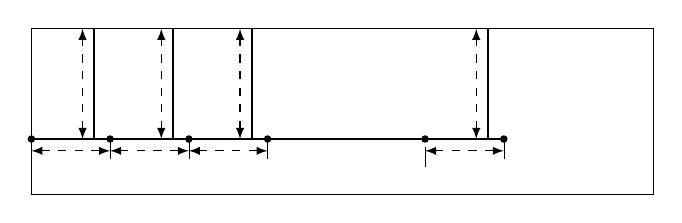
\begin{tikzpicture}[>=latex]
\draw (0.3,0.2) rectangle +(7.9,2.1);
\draw[thick] (0.3,0.9) -- ++(6,0);
\foreach \x/\y in {1/1,2/2,3/3,6/{n}}
{
    \draw[thick] (\x + 0.1,0.9) -- ++(0,1.4);
    \filldraw[black] (\x + 0.3,0.9) circle(0.04);
    \draw[ultra thin] (\x + 0.3,0.9) -- ++ (0,-0.25);
    \draw[<->,dashed] (\x - 0.7,0.75) to node [label=below:{\small }] {} (\x + 0.3,0.75);
    \draw[<->,dashed] (\x - 0.05,0.9) to node [label=left:{\small }] {} (\x - 0.05,2.3);
}
\filldraw[black] (0.3,0.9) circle(0.04);
\filldraw[black] (5.3,0.9) circle(0.04);
\draw[ultra thin] (5.3,0.8) -- ++ (0,-0.25);
\end{tikzpicture}
\end{center}
\vspace*{-2mm}
\caption{Encoding the PCP: Stage 1.}
\label{fig:Summary1}
\end{figure}
These arcs define a `window,' containing a sequence  of
`horizontal' arcs (), each connected by a
corresponding `vertical arc,' , to some point on the `top
edge.' We can ensure that each  is included in a region
, and each  () in a region
, where  now indicates . By
repeating the construction, a second pair of arc-sequences,
 and  () can be
established, but with each  connecting  to the
`bottom edge.' Again, we can ensure each  is included in a
region  and each  in a region  (). Further, we can ensure that the final horizontal arcs
 and  (but no others) are joined by an arc
 lying in a region .
\begin{figure}[h]
\centering
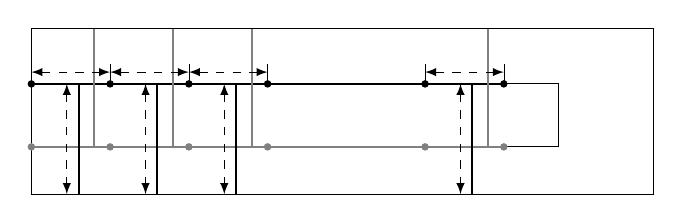
\begin{tikzpicture}[>=latex]
\draw (0.3,0.2) rectangle +(7.9,2.1);
\draw[gray,thick] (0.3,0.8) -- ++(6,0);
\draw (6.3,1.6) -- (7,1.6) -- (7,0.8) -- (6.3,0.8);
\draw[thick] (0.3,1.6) -- ++(6,0);
\foreach \x/\y in {1/1,2/2,3/3,6/{n}}
{
    \draw[thick,gray] (\x + 0.1,0.8) -- ++(0,1.5);
    \draw[thick] (\x - 0.1,0.2) -- ++(0,1.4);
    \filldraw[gray] (\x + 0.3,0.8) circle(0.04);
    \filldraw[black] (\x + 0.3,1.6) circle(0.04);
    \draw[ultra thin] (\x + 0.3,1.6) -- ++ (0,0.25);
    \draw[<->,dashed] (\x + 0.3,1.75) to node [label=above:{\footnotesize }] {} (\x - 0.7,1.75);
    \draw[<->,dashed] (\x - 0.25,1.6) to node {} (\x - 0.25,0.2);
    \node at (\x-0.45,1.15) {{\footnotesize }};
}
\filldraw[gray] (0.3,0.8) circle(0.04);
\filldraw[gray] (5.3,0.8) circle(0.04);
\filldraw[black] (0.3,1.6) circle(0.04);
\filldraw[black] (5.3,1.6) circle(0.04);
\draw[ultra thin] (5.3,1.6) -- ++ (0,0.25);
\node (last) at (6.9,1.3) [label=right:{\small }] {};
\end{tikzpicture}
\caption{Encoding the PCP: Stage 2.}
\label{fig:Summary2}
\end{figure}
The crucial step is to match up these arc-sequences.  To do so, we
write , for all ,  (, ). A simple argument based on planarity considerations then ensures
that the upper and lower sequences of arcs must cross (essentially) as
shown in Fig.~\ref{fig:Summary2}. In particular, we are guaranteed
that  (without specifying the value ), and that, for all ,  is connected by  (and also by
) to .


Having established the configuration of Fig.~\ref{fig:Summary2}, we
write , for , ensuring that each  is included in
exactly one of , . These inclusions naturally define a word
 over the alphabet .  Next, we write
-constraints which organize the sequences of arcs
 and  (independently) into consecutive
blocks. These blocks of arcs can then be put in 1--1 correspondence
using essentially the same construction used to put the individual
arcs in 1--1 correspondence. Each pair of corresponding blocks can now
be made to lie in exactly one region from a collection . We think of the  as representing the letters of the
alphabet , so that the labelling of the blocks with these elements
defines a word . It is then straightforward to write
non-contact constraints involving the arcs  ensuring that
 and non-contact constraints involving the arcs
 ensuring that . Let  be the
conjunction of all the foregoing -formulas. Thus, if 
is satisfiable over , then  is a positive instance of
the PCP. On the other hand, if  is a positive instance of the
PCP, then one can construct a tuple satisfying  over
 by `thickening' the above collections of arcs into
polygons in the obvious way. So,  is positive iff  is
satisfiable over  iff  is satisfiable over
. This shows r.e.-hardness of  and
.  Membership of the latter problem in r.e.~is
immediate because all polygons may be assumed to have vertices with
rational coordinates, and so may be effectively enumerated.  Using the
techniques of Corollaries~\ref{cor:inftyCci}--\ref{cor:inftyBc} and
Theorem~\ref{theo:inftyBci}, we obtain:
\begin{theorem}
\label{theo:undecidable}
For ,
 is r.e.-hard, and
 is r.e.-complete.
\end{theorem}

The complexity of  remains open for the
languages . However, as we
shall see in the next section, for  it drops dramatically.





\section{\cBci{} in 3D}\label{sec:3d}

In this section, we consider the complexity of satisfying
\cBci-constraints by polyhedra and regular closed sets in
three-dimensional Euclidean space. Our analysis rests on an important
connection between geometrical and graph-theoretic interpretations. We
begin by briefly discussing the results of~\cite{ijcai:kp-hwz10} for
the {\em polyhedral} case.

Recall that every partial order , where  is a transitive and
reflexive relation on , can be regarded as a topological space by
taking  to be open just in case  and 
imply . Such topologies are called \emph{Aleksandrov spaces}.
If  contains no proper paths of length greater than 2, we call
 a \emph{quasi-saw} (Fig.~\ref{fig:broom}).  If, in
addition, no  has more than two proper -successors, we
call  a \emph{-quasi-saw}.  The properties of 2-quasi-saws
we need are as follows~\cite{ijcai:kp-hwz10}:
\begin{itemize}\itemsep=0pt
\item[--] satisfiability of -formulas in arbitrary topological
  spaces coincides with satisfiability in 2-quasi-saws, and is
  \ExpTime-complete;

\item[--]  is connected in a 2-quasi-saw  iff it is interior-connected in .
\end{itemize}
The following construction lets us apply these results to the problem
.  Say that a \emph{connected partition} in
 is a tuple  of non-empty polyhedra having
connected and pairwise disjoint interiors, which sum to the entire
space . The \emph{neighbourhood graph}  of this partition
has vertices  and edges 
(Fig.~\ref{fig:conn-part}).
\begin{figure}[h]
\begin{center}
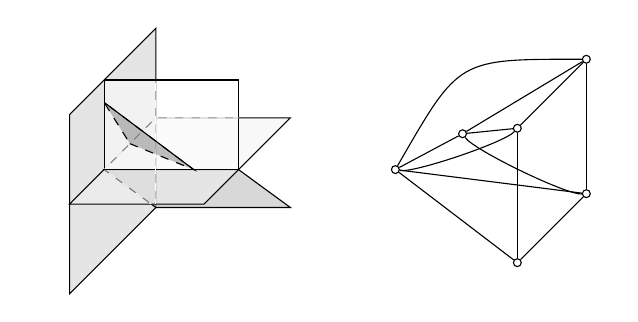
\begin{tikzpicture}[point/.style={circle,draw=black,minimum size=1mm,inner sep=0pt},scale=0.2mm]
\filldraw[fill=Gray!20] (0,-2,-3) -- (0,2,-3) -- (0,2,2) -- (0,-2,2) --   cycle;
\filldraw[fill=Gray!60,fill opacity=0.5] (0,0,0) -- (3,0,0) -- (3,-2,-3) -- (0,-2,-3) --   cycle;
\filldraw[fill=Gray!10,fill opacity=0.5] (0,0,-3) -- (0,0,2) -- (3,0,2) -- (3,0,-3) --   cycle;
\filldraw[fill=white,fill opacity=0.5] (0,0,0) -- (3,0,0) -- (3,2,0) -- (0,2,0) --   cycle;
\begin{scope}[dashed,draw=white]
\clip (0,0,0) -- (3,0,0) -- (3,2,0) -- (0,2,0) --   cycle;
\draw (0,-2,-3) -- (0,2,-3);
\draw (0,0,2) -- (0,0,-3) -- (3,0,-3);
\end{scope}
\begin{scope}[dashed,draw=white]
\clip (0,0,-3) -- (0,0,2) -- (3,0,2) -- (3,0,-3) --   cycle;
\draw (0,-2,-3) -- (0,2,-3);
\draw (0,-2,-3) -- (0,0,0);
\end{scope}
\filldraw[dashed,fill=Gray,fill opacity=0.5] (0,0,-1.5) -- (2,0,0) -- (0,1.5,0)  --   cycle;
\draw (2,0,0) -- (0,1.5,0);
\node (1) at (-1.5,0,0) {\small };
\node (2) at (1.8,-1,1.5) {\small };
\node (3) at (3,-1,-2.5) {\small };
\node (4) at (1.8,1.5,-2.5) {\small };
\node (5) at (2.5,.5,2) {\small };
\node (6) at (0.3,0.3,-0.3) {\small };
\begin{scope}[xshift=80mm]
\node [label=left:{\small }] (v1) at (-1.5,0,0) [point] {};
\node [label=right:{\small }](v2) at (1.8,-1.5,1.5)[point] {};
\node [label=right:{\small }](v3) at (1.8,-1.5,-2.5)[point] {};
\node [label=right:{\small }](v4) at (1.8,1.5,-2.5)[point] {};
\node [label=right:{\small }](v5) at (1.8,1.5,1.5)[point] {};
\node [label=above:{\small }] (v6) at (0,0.8,0)[point] {};
\draw (v1) -- (v2);
\draw (v2) -- (v3);
v\draw (v1) -- (v3);
\draw (v3) -- (v4);
\draw (v2) -- (v5);
\draw (v1) to [bend right, looseness=0.3] (v5);
\draw (v1) to [bend left, looseness=1.5] (v4);
\draw (v3) to [bend left, looseness=0.3] (v6);
\draw (v4) -- (v5);
\draw (v1) -- (v6);
\draw (v4) -- (v6);
\draw (v5) -- (v6);
\end{scope}
\end{tikzpicture}
\end{center}
\vspace*{-2mm}
\caption{A connected partition and its neighbourhood graph.}\label{fig:conn-part}
\end{figure}
One can show that {\em every} 
connected graph is the neighbourhood graph of
some connected partition in . Furthermore, every
neighbourhood graph  gives rise to a 2-quasi-saw, namely, , where , , and  is the reflexive closure of . From this, we see that ({\em i}) a
-formula  is satisfiable over  iff ({\em
  ii})  is satisfiable over a connected -quasi-saw iff ({\em
  iii}) the -formula , obtained from  by
replacing every occurrence of  with , is satisfiable over a
connected 2-quasi-saw. Thus,  is
\ExpTime-complete.

The picture changes if we allow variables to range over 
rather than . Note first that the -formula
\eqref{eq:wiggly} is not satisfiable over 2-quasi-saws, but has a
quasi-saw model as in Fig.~\ref{fig:broom}.
\begin{figure}[ht]
\centering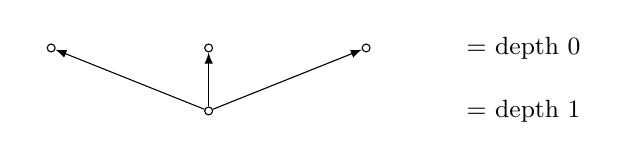
\begin{tikzpicture}[>=latex, point/.style={circle,draw=black,minimum size=1mm,inner sep=0pt}]
\node (r1) at (2,0.8)  [point,label=left:{}] {};
\node (r2) at (4,0.8)  [point,label=right:{}] {};
\node (r3) at (6,0.8)  [point,label=right:{}] {};
\node (r) at (4,0)  [point,label=below:{}] {};
\draw[->] (r) to node [below] {\scriptsize } (r1);
\draw[->] (r) to node [right] {\scriptsize } (r2);
\draw[->] (r) to node [below] {\scriptsize } (r3);
\node at (8,0) {\small  = depth 1};
\node at (8,0.8) {\small  = depth 0};
\end{tikzpicture}
\vspace*{-3mm}
\caption{A quasi-saw model  of~\eqref{eq:wiggly}: .}
\label{fig:broom}
\end{figure}
Some extra geometrical work will show now that ({\em iv}) a
-formula is satisfiable over  iff ({\em v}) it is
satisfiable over a connected quasi-saw.  And as shown
in~\cite{ijcai:kp-hwz10}, satisfiability of -formulas in
connected spaces coincides with satisfiability over connected
quasi-saws, and is \NP-complete.
\begin{theorem}\label{theo:BciRCR3}
The problem  is \NP-complete.
\end{theorem}
\begin{proof}
From the preceding discussion, it suffices to show that ({\em v})
implies ({\em iv}) for any -formula . So suppose
, with  based on a finite
connected quasi-saw , where  contains all points
of depth  (Fig.~\ref{fig:broom}).  Without loss of
generality we will assume that there is a special point  of depth
1 such that  for all  of depth 0.  We show how
 can be embedded into .

Take pairwise disjoint \emph{closed} balls , for  of depth
0, and pairwise disjoint \emph{open} balls , for all  of depth
1 except  (we assume the  are disjoint from the
). Let  be the closure of the complement of all
 and .


We expand the  to sets  in such a way that
\begin{itemize}\itemsep=0pt
\item[(A)] the  form a connected partition in , that
  is, they are regular closed and sum up to , and their
  interiors are non-empty, connected and pairwise disjoint;

\item[(B)] every point in  is either
in the interior of some  with , or on the boundary of \emph{all} of the  with .
\end{itemize}
The required  are constructed as follows.
Let  be an enumeration of all the points in the interiors of  with \emph{rational} coordinates.
For , we set  to be the closure of the infinite union
, where the regular closed sets
 are defined inductively as follows (Fig.~\ref{fig:apollonian}).
Assuming that the  are defined, let  be the first point in
the list  that is not in any  yet. So,  is in the interior of some . Take an open ball
 in the interior of  centred in  and
disjoint from the . For each  with , expand
 by a closed ball in  and a closed `rod' connecting it
to  in such a way that the ball and the rod are disjoint from
the rest of the ; the result is denoted by .
\begin{figure}[h]
\begin{center}
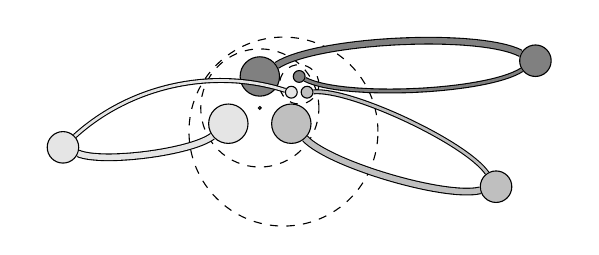
\begin{tikzpicture}[clball/.style={circle,draw=black,minimum size=4mm,inner sep=0pt},
opball/.style={circle,dashed,draw=black,minimum size=25mm,inner sep=0pt}]
\node [label=left:{\small }] (x1) at (0,-3)[clball,fill=Gray!20] {};
\node [label=right:{\small }] (x2) at (6,-1.9)[clball,fill=Gray] {};
\node [label=right:{\small }] (x3) at (5.5,-3.5)[clball,fill=Gray!50] {};
\node [label=below left:{\small }] (z1) at (2.8,-2.8)[opball,minimum size=24mm] {};
\node [label=below:{\small }](c) at (2.5,-2.5)[opball,minimum size=15mm] {};
\node [label=below:{\small }](q) at (2.5,-2.5)[circle,inner sep=0pt,minimum size=1,draw=black] {};
\node (xc1) at (2.1,-2.7)[clball,fill=Gray!20,minimum size=5mm] {};
\node (xc2) at (2.5,-2.1)[clball,fill=Gray,minimum size=5mm] {};
\node (xc3) at (2.9,-2.7)[clball,fill=Gray!50,minimum size=5mm] {};
\draw[double=Gray!20,double distance=2pt] (xc1) to [bend left, looseness=0.5] (x1);
\draw[double=Gray,double distance=2pt] (xc2) to [bend left, looseness=0.5] (x2);
\draw[double=Gray!50,double distance=2pt] (xc3) to [bend right, looseness=0.5] (x3);
\node (cp) at (3,-2.2)[opball,minimum size=5mm] {};
\node (xcp1) at (2.9,-2.3)[clball,fill=Gray!20,minimum size=1.5mm] {};
\node (xcp2) at (3,-2.1)[clball,fill=Gray,minimum size=1.5mm] {};
\node (xcp3) at (3.1,-2.3)[clball,fill=Gray!50,minimum size=1.5mm] {};
\draw[double=Gray!20,double distance=1pt] (xcp1) to [bend right, looseness=0.9] (x1);
\draw[double=Gray,double distance=1pt] (xcp2) to [bend right, looseness=0.5] (x2);
\draw[double=Gray!50,double distance=1pt] (xcp3) to [bend left, looseness=0.5] (x3);
\end{tikzpicture}
\end{center}
\vspace*{-2mm}
\caption{Filling  with , for , .}\label{fig:apollonian}
\end{figure}
Consider a function  that maps regular closed sets  to
 so that  is the union of all , for  of depth
 in .  By~(A),  preserves , , ,  and .
Define an interpretation  over  by
. To show that , it remains to prove that  is connected iff
 is connected (details are in Appendix~\ref{sec:Bci3D_C}).
\end{proof}



The remarkably diverse computational behaviour of \cBci{} over
,  and  can be explained as
follows. To satisfy a \cBci-formula  in , it suffices
to find polynomially many points in the regions mentioned in 
(witnessing non-emptiness or non-internal-connectedness constraints),
and then to `inflate' those points to (possibly internally connected)
regular closed sets using the technique of Fig.~\ref{fig:apollonian}.
By contrast, over , one can write a \cBci-formula
analogous to \eqref{eq:contactTrick} stating that two internally
connected polyhedra do not share a 2D face.  Such
`face-contact' constraints can be used to generate constellations of
exponentially many polyhedra simulating runs of alternating Turing
machines on polynomial tapes, leading to \ExpTime-hardness. Finally,
over , planarity considerations endow \cBci{} with the
extra expressive power required to enforce full non-contact constructs
(not possible in higher dimensions), and thus to encode the PCP as
sketched in Sec.~\ref{sec:undecidability}.







\section{Conclusion}\label{conclusion}

This paper investigated topological constraint
languages featuring connectedness predicates and Boolean operations on
regions.  Unlike their less expressive cousins, \RCCE{} and \RCCF,
such languages are highly sensitive to the spaces over which they
are interpreted, and exhibit more challenging computational
behaviour. Specifically, we demonstrated that the languages ,
 and  contain formulas satisfiable over , , but only by regions with infinitely many components. Using a
related construction, we proved that the satisfiability problem for
any of , ,  and , interpreted either over
 or over its polygonal subalgebra, , is
\emph{undecidable}. Finally, we showed that the satisfiability problem
for , interpreted over , is \NP-complete, which
contrasts with \ExpTime-completeness for .  The complexity
of satisfiability for ,  and  over  or
 for  remains open. 
The obtained results rely on certain
distinctive topological properties of Euclidean spaces. 
Thus, for example, the argument of
Sec.~\ref{sec:sensitivity} is based on the property of
Lemma~\ref{lma:ourNewman}, while Sec.~\ref{sec:undecidability}
similarly relies on {\em planarity} considerations. In both cases,
however, the moral is the same: the topological spaces of most
interest for Qualitative Spatial Reasoning exhibit special
characteristics which any topological constraint language able to
express connectedness must take into account.

The results of Sec.~\ref{sec:undecidability} pose a challenge for
Qualitative Spatial Reasoning in the Euclidean plane.  On the one hand, the
relatively low complexity of \RCCE{} over disc-homeomorphs suggests
the possibility of usefully extending the expressive power of \RCCE{}
without compromising computational properties. On the other hand, our
results impose severe limits on any such extension.  We observe,
however, that the constructions used in the proofs depend on a strong
interaction between the connectedness predicates and the Boolean
operations on regular closed sets. We believe that by restricting this
interaction one can obtain non-trivial constraint languages with more
acceptable complexity. For example, the extension of \RCCE{} with
connectedness constraints is still in \NP{} for both  and
~\cite{ijcai:kphz10}.


\smallskip
\noindent
{\bf Acknowledgments.}\ \ This work was partially supported by the U.K. EPSRC grants EP/E034942/1 and EP/E035248/1.



\bibliographystyle{named}



\begin{thebibliography}{}\itemsep=1pt



\bibitem[\protect\citeauthoryear{Bennett}{1994}]{ijcai:Bennett94}
B.~Bennett.
\newblock Spatial reasoning with propositional logic.
\newblock In {\em Proc.\ of KR}, pages 51--62.  1994.

\bibitem[\protect\citeauthoryear{Borgo \bgroup \em et al.\egroup
  }{1996}]{Borgo96}
S.~Borgo, N.~Guarino, and C.~Masolo.
\newblock A pointless theory of space based on strong connection and
  congruence.
\newblock In {\em Proc.\ of
  KR}, pages 220--229. 1996.

\bibitem[\protect\citeauthoryear{Cohn and Renz}{2008}]{ijcai:Cohn&Renz08}
A. Cohn and J. Renz.
\newblock Qualitative spatial representation and reasoning.
\newblock In {\em
  Handbook of Kno\-w\-ledge Representation}, pages 551--596. Elsevier, 2008.

\bibitem[\protect\citeauthoryear{Dornheim}{1998}]{Dornheim}
C.\ Dornheim.
\newblock Undecidability of plane po\-ly\-gonal mereo\-topology.
\newblock In {\em Proc.\ of KR}. 1998.


\bibitem[\protect\citeauthoryear{Egenhofer and
  Franzosa}{1991}]{ijcai:Egenhofer&Franzosa91}
M.~Egenhofer and R.~Franzosa.
\newblock Point-set topological spatial relations.
\newblock {\em International J.\ of Geographical Information Systems},
  5:161--174, 1991.



\bibitem[\protect\citeauthoryear{Kontchakov \bgroup \em et al.\egroup
  }{2010a}]{ijcai:kp-hwz10}
R.~Kontchakov, I.~Pratt-Hartmann, F.~Wolter, and M.~Zakharyaschev.
\newblock Spatial logics with connectedness predicates.
\newblock {\em Logical Methods in Computer Science}, 6(3), 2010.

\bibitem[\protect\citeauthoryear{Kontchakov \bgroup \em et al.\egroup
  }{2010b}]{ijcai:kphz10}
R.~Kontchakov, I.~Pratt-Hart\-mann, and M.~Zakharyaschev.
\newblock Interpreting topological logics over {E}uclidean spaces.
\newblock In {\em Proc.\
  of KR}. 2010.

\bibitem[\protect\citeauthoryear{Newman}{1964}]{ijcai:Newman64}
M.H.A. Newman.
\newblock {\em Elements of the Topology of Plane Sets of Points}.
\newblock Cambridge, 1964.

\bibitem[\protect\citeauthoryear{Pratt-Hartmann}{2007}]{ijcai:HSL2}
I.~Pratt-Hartmann.
\newblock First-order mere\-o\-topology.
\newblock In {\em
  Handbook of Spatial Logics}, pages 13--97. Springer, 2007.

\bibitem[\protect\citeauthoryear{Randell \bgroup \em et al.\egroup
  }{1992}]{ijcai:Randelletal92}
D.~Randell, Z.~Cui, and A.~Cohn.
\newblock A spatial logic based on regions and connection.
\newblock In {\em Proc.\ of
  KR}, pages 165--176. 1992.

\bibitem[\protect\citeauthoryear{Renz and Nebel}{2001}]{ijcai:Renz&Nebel98}
J.~Renz and B.~Nebel.
\newblock Efficient methods for qualitative spatial reasoning.
\newblock {\em J.~Artificial Intelligence Research}, 15:289-318, 2001. 
\bibitem[\protect\citeauthoryear{Renz}{1998}]{ijcai:Renz98}
J.~Renz.
\newblock A canonical model of the region connection calculus.
\newblock In {\em Proc.\ of
  KR},`pages 330--341. 1998.

\bibitem[\protect\citeauthoryear{Schaefer \bgroup \em et al.\egroup
  }{r003}]{ijcai:iscloes:sss03}
M.~Schaefer, E.~Sedgwick, and D.~{\v{S}}tefankovi{\v{c}}.
\newblock Recognizing string graphs in {NP}.
\newblock {\em J.\ of Computer and System Sciences}, 67:365--380, 2003.

\bibitem[\protect\citeauthoryear{Wolter and
  Zakharyaschev}{2000}]{ijcai:Wolter&Z00ecai}
F.~Wolter and M.~Zakharyaschev.
\newblock Spatial reasoning in \RCCE{} with {B}oolean region terms.
\newblock In {\em Proc.\ of ECAI}, pages 244--248.  2000.

\end{thebibliography}

\cleardoublepage

\appendix

\section{Regions with infinitely many components}
\label{sec:sensitivityA}
First we give detailed proofs of Lemma~\ref{lma:ourNewman} and
Theorem~\ref{theo:inftyCc}.
\begin{theorem}[\cite{ijcai:Newman64}]\label{thm:NewmanBnd} 
If  is a connected subset of , then every connected component
of  has a connected boundary.
\end{theorem}

\begin{swetheorem}{Lemma~\ref{lma:ourNewman}}
If  is connected, then every component of  has a
connected boundary.
\end{swetheorem}
\begin{proof}
Let  be a connected component of .  Suppose that the boundary
 of  is not connected, and let  and  be
two sets separating :  and  are disjoint,
non-empty, closed subsets of  whose union is . We will
show that  is not connected.  We have , for some index set , where the  are distinct
connected components of .  By
Theorem~\ref{thm:NewmanBnd},`the boundaries  of  are
connected subsets of , for each . Hence, either
 or , for
otherwise  and  would
separate . Let  and , for .
Clearly,  and  are closed, and . Hence, it
suffices to show that  and  are disjoint. We know that, for
,

Clearly,  and  are disjoint. We also know that 
 and  are disjoint, as 
subsets of  and , respectively. Finally,  
and  are disjoint, for , as subsets of the boundary and the 
interior of , respectively. So,  is not connected, which is a contradiction.
\end{proof}

\begin{swetheorem}{Theorem~\ref{theo:inftyCc}}
	If  is an interpretation over  such that
	, then every 
	has infinitely many components.
\end{swetheorem}
\begin{proof}
To simplify presentation, we ignore the difference  between variables and the regions 
they stand for, writing, for example,  instead of . We also set 
. We construct a sequence of disjoint components  of  
and open sets  connecting  to  (Fig.~\ref{fig:InfCmpConstr}). By the first 
conjunct of~\eqref{eq:basic-regions}, let  be a component of  containing points in 
. Suppose  has been constructed, for . By~\eqref{eq:InfContact} 
and~\eqref{notC}, there exists a point . Since 
, and because  is locally connected, 
there exists a connected neighbourhood  of  such that 
, and so, 
by~\eqref{eq:InfPart1}, . Further, since ,
. Take  to be a component of  that 
intersects  and  the component of  containing .
	
To see that the  are distinct, let  and  be the
components of  containing  and ,
respectively. It suffices to show .
Note that the connected set  must intersect .
Evidently, .
Also, ; hence,
by~\eqref{eq:InfPart1} and~\eqref{eq:InfNTriv1}, .  By Lemma~\ref{lma:ourNewman},
 is connected, and therefore, by~\eqref{eq:InfNTriv1},
is entirely contained either in  or in
. Since  and
, we have , so . Similarly,
.  By~\eqref{eq:InfNTriv1}, then,
, and since 
and  are components of the same set, they are
disjoint. Hence, , and since
, also . So,  lies in the interior of
a component of , and since , that component must be .
\end{proof}


Now we extend the result to the language . All occurrences of
 in  have positive polarity.  Let 
be the result of replacing them with the predicate . In the
configuration of Fig.~\ref{fig:InfCmpSat}, all connected regions
mentioned in  are in fact interior-connected; hence
 is satisfiable over . Since
interior-connectedness implies connectedness, 
entails  in a common extension of  and
. Hence:
\begin{swetheorem}{Corollary~\ref{cor:inftyCci}}
There is a -formula satisfiable over , ,
but not by regions with finitely many components.
\end{swetheorem}
\begin{figure}[h]
\begin{center}
\begin{tikzpicture}
\scriptsize{
	\coordinate (Px) at (-3.8,0);
	\coordinate (Qx) at (-3.3,0);
	\coordinate (Py) at (0,1.3);
	\coordinate (Pty) at (0.23,-.9);
	\coordinate (Pby) at (0,1);
	\foreach \i/\a/\b in {2/20/0,1/10/0,0/0/30,3/0/0,2/20/0,1/10/0,0/0/30}
	{
		\draw[fill=black!\a] () rectangle ();		
		\draw[fill=black!\b] () rectangle ();
		\node at () {};
		\node at () {};		
		
		\coordinate (Px) at ();
		\coordinate (Py) at ();
		\coordinate (Pty) at ();
		\coordinate (Pby) at ();
		\coordinate (Qx) at ();
	}
	\draw (4.3,0.5)--(.5,0.25)--(.5,0.2)--(4.3,0.2);
	\node at (4.1,.35) {};
	\node at (4.1,0) {};
	\draw (-4.3,0.25)--(-.75,0)--(-.75,-0.05)--(-4.3,-0.05);
	\node at (-4.1,.125) {};
}
\end{tikzpicture}	
\end{center}
	\caption{Satisfying  and .}
	\label{fig:InfCmpElAiBi}	
\end{figure}
To extend Theorem~\ref{theo:inftyCc} to the language , 
notice that all occurrences of  in  are negative.
We shall eliminate these using only the predicate . We use
the fact that, if the sum of two connected regions is not 
connected, then they must be disjoint. Consider the formula 

Note that  implies .  We
replace  with , which is clearly satisfiable by the
regions on Fig.~\ref{fig:InfCmpSat}. Further, we replace  with . As shown
on Fig.~\ref{fig:InfCmpElAiBi}, there exists a region  satisfying
this formula.  Instead of dealing with , we
consider the equivalent:

We replace  by ,
which is satisfiable by the regions depicted on Fig.~\ref{fig:InfCmpElAiBi}.
We ignore , because it is logically equivalent to 
, for different values of . We replace 
 by , 
which is satisfiable by the regions depicted on Fig.~\ref{fig:InfCmpElAiAi2}. The fourth 
conjunct is then treated symmetrically.
\begin{figure}[h]
\begin{center}
\begin{tikzpicture}
\scriptsize{
	\node at (-5.2,0) {};
	\clip (-5,-2) rectangle (2.5,2);
	\coordinate (Px) at (-4.8,0);
	\coordinate (Qx) at (-4.3,0);
	\coordinate (Py) at (0,1.7);
	\coordinate (Pty) at (0.23,0);
	\coordinate (Pby) at (0,1.4);
	\coordinate (Q0) at (-4.8,-1.4);
	\coordinate (Q2) at (-4.8,1.4);
	
	\foreach \i/\a/\b in {0/0/30,3/0/0,2/0/10,1/0/0,0/0/30,3/0/0,2/0/10,1/0/0,0/0/30}
	{
		\draw[fill=black!\a,draw=gray] () rectangle ();		
		\draw[fill=black!\b,draw=gray] () rectangle ();
		\node at () {};
		\node at () {};		
		\ifnum \i=0
			\draw[fill=black!30]  () to[out=-135,in=-45]  
			()--++(-.2,0) to[out=-60,in=-135] ()
			node[very near end, below]{}--cycle;
		\fi
		\ifnum \i=2
			\draw[fill=black!10]  () to[out=135,in=45]  
			()--++(-.2,0) to[out=60,in=135] ()
			node[very near end, above]{}--cycle;
		\fi
		\coordinate (Px) at ();
		\coordinate (Py) at ();
		\coordinate (Q0) at ();
		\coordinate (Q2) at ();
\coordinate (Pby) at ();
		\coordinate (Qx) at ();
	}
	\draw (4.3,0.5)--(.5,0.25)--(.5,0.2)--(4.3,0.2);
	\node at (4.1,.35) {};
	\node at (4.1,0) {};	
}
\end{tikzpicture}		
\end{center}
	\caption{Satisfying .}
	\label{fig:InfCmpElAiAi2}	
\end{figure}
Transforming  in the way just described, we obtain a
-formula , which implies  (in the
language ) and which is satisfiable by the arrangement of
. Hence, we obtain the following:
\begin{swetheorem}{Corollary~\ref{cor:inftyBc}} 
There is a -formula satisfiable over , ,
but not by regions with finitely many components.
\end{swetheorem}

The only remaining task in this section is to prove Theorem~\ref{theo:inftyBci}.
The construction is similar to the one developed in Sec.~\ref{sec:undecidability},
and as such uses similar techniques. We employ the following notation. 
If  is a Jordan arc, and ,  are points on  such that 
 occurs after , we denote by  the segment of  from 
 to .
Consider the formula  given by:

This formula allows us to construct sequences of arcs in the following
sense:
\begin{lemma}\label{lma:StackLemmai} 
Suppose that the condition  obtains,
. Then every point  can be connected to every
point  by a Jordan arc
 such that for all  \textup{(}\textup{)}, each segment  is a
non-degenerate Jordan arc starting at some point .
\end{lemma}
\begin{proof}
	By , let  be a Jordan arc connecting  to
         (Fig.~\ref{fig:stacki}). By the non-contact constraints,
         has to contain points in . Let  be
        one such point.  For  we suppose ,  and  to have been
        defined, and proceed as follows. By , let
         be a Jordan arc
        connecting  to . By the non-contact constraints,
         can intersect
         only in its final
        segment . Let  be the first point of
         lying on ; let  be
        the initial segment of  ending at ;
        and let  be the final segment of 
        starting at . It remains only to define
        , and to this end, we simply set
        . To see that , ,
        are as required, note that . By the disjoint constraints 
        must be in . If  was in , it would also
        have to be in  and , which
        is forbidden by the disjoint constraints. Hence , . Given , , this also guarantees that the arcs  are
        non-degenerate.
\end{proof}
\begin{figure}[h]\begin{center}
	\begin{tikzpicture}
		\scriptsize
		{
			\draw[very thick] (1,2) circle(1pt) node[below]{}--
					(2,2) circle (1pt) node[above left]{} node[below,midway]{};
			\draw[dotted,-latex] (3,2)--(4,2) node[above,midway]{};
			\draw[ultra thin,-latex,shorten >=1pt] (3,2) node[below]{} 
					to[out=90,in=90] (2,2) node[above,midway]{};
			\fill[ultra thin] (3,2) circle(1pt);
			\draw[ultra thin] (3,2) --(2,2) node[below,midway]{};
			
			\draw[very thick,-latex] (2,2) to[out=-70,in=180] (3.3,1.2) node[midway,below]{};
			\begin{scope}[xshift=-.5cm]
				\node at (4.2,1.2) {{\normalsize }};
				
				\draw[very thick] (4.6,1.2) -- (5.7,1.2) node[midway,below]{} 
						node[above left]{} circle(1pt);
				\draw[ultra thin] (5.7,1.2)--(7,1.2) circle(1pt) node[above]{};
				\draw[dotted,-latex](7,1.2)--++(1,0) node[below,midway]{};
				\draw[ultra thin,-latex,shorten >=1pt] (7,1.2) to[out =-90,in=-90]
								(5.7,1.2) node[midway,below]{};
				\draw[very thick,-latex,shorten >=1pt] (5.7,1.2) to[out=90,in=180] 
					(8,2) node[above]{} node[midway,above]{};
				\fill[very thick] (8,2) circle(1pt);
			\end{scope}
		}
	\end{tikzpicture}
\end{center}
\caption{The constraint  ensures the existence of a Jordan arc 
 which connects a point  to a point .}
\label{fig:stacki}
\end{figure}


Consider now the formula  given by:

where  denotes .  This formula allows us to
construct Jordan curves in the plane, in the following sense:
\begin{lemma}\label{lma:FrameLemmaInt}
	Let , and suppose .
        Then there exist Jordan arcs , \ldots, 
        such that  is a Jordan curve lying in
        the interior of , and , for all , .
\end{lemma}
\begin{proof}
For all  (), pick , and pick a Jordan arc
 from  to .  
For all  (), let  be the first point
of  lying on , and let  be the
first point of  lying on . For all  (), let , let , and let  denote the section of
 (in the appropriate direction) from  to . Now
let  be the first point of  lying on
, let , and let . It is routine to verify that the arcs
, \ldots,  have the required properties.
\end{proof}

We will now show how to separate certain types of regions in the language . 
We make use of Lemma~\ref{lma:FrameLemmaInt} and the following fact.
\begin{lemma}\label{lma:Newman}{\cite[p.~137]{ijcai:Newman64}}
	Let ,  be disjoint, closed subsets of  such that
	 and  are connected. Then
	 is connected.
\end{lemma}
\begin{figure}[h]
	\begin{center}
		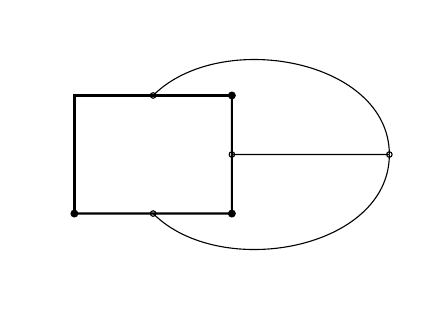
\begin{tikzpicture}
		\scriptsize{
			\draw[black,thick] (0,0)--++(0,1.5)--++(2,0);
			\filldraw[black,thick] (0,0) circle(1pt) --++ (2,0) circle(1pt);
			\filldraw[black,thick] (2,0)--(2,1.5) circle(1pt);
			
			\draw (4,.75) node[right]{} circle(1pt)--
				(2,.75) circle(1pt) node[left]{} node[midway,above]{};
			\draw (4,.75) to[out=90,in=45] 
				(1,1.5) circle(1pt) node[below]{} node[midway,above]{};
			\draw (4,.75) to[out=-90,in=-45] 
				(1,0) circle(1pt) node[above]{} node[midway,below]{};;
			
			\node at (.4,-.2){};
			\node at (.3,1.7){};
			\node at (2.2,1.1){};
			
			\node at (-.5,.75) {};
			\node at (2.6,1.4) {};
			\node at (2.6,0) {};
		}	
	\end{tikzpicture}
	\end{center}
	\caption{The Jordan curve  separating  from .}
	\label{fig:SepBci}
\end{figure}
We say that a region  is \emph{quasi-bounded} if either  or  is bounded.
We can now prove the following.
\begin{lemma}\label{lma:Cci2BciStar}
	There exists a -formula  with the
	following properties: \textup{(}i\textup{)} 
	entails  over ; \textup{(}ii\textup{)}
	if the regions  and  can be separated by a Jordan curve, 
	then there exist polygons  such that 
	; \textup{(}iii\textup{)} if ,
	 are disjoint polygons such that  is quasi-bounded and
	 is connected, then there exist polygons
	 such that .
\end{lemma}
\begin{proof}
	Let  be the tuple of variables , and let
	 be the formula
	
	
	Property ({\em i}) follows by a simple planarity argument. By
	 and Lemma~\ref{lma:FrameLemmaInt}, 
	let , for , be such that 
	 is a Jordan curve included in 
	. Further, let 
	,  
	(Fig.\ref{fig:SepBci}). Note that all points in ,
	, that are on  are on . By 
	, , let 
	 be a Jordan arc with 
	endpoints  and . 
	We may assume that these arcs intersect only at their common 
	endpoint , so that they divide the residual domain of 
	 which contains  into three sub-domains , for 
	. The existence of a point  in any 
	, , will contradict . 
	So,  must be contained entirely in the residual domain of 
	 not containing . Similarly, all points in  must 
	lie in the residual domain of  containing . It follows 
	that  and  are disjoint, and by  and 
	, that  and  are disjoint as well.
	For Property ({\em ii}), let  be a Jordan curve
	separating  and . Now thicken  to form an annular
	element of , still disjoint from  and , and divide
	this annulus into the three regions  as shown
	(up to similar situation) in Fig.~\ref{fig:Cci2BciStar}.
	Choose  and  to be the connected components
	of  containing  and , respectively.	
	For Property ({\em iii}), it is routine using Lemma~\ref{lma:Newman} 
	to show that there exists a piecewise linear Jordan curve
	  in  separating  and .
\end{proof}

\begin{figure}[h]
\begin{center}
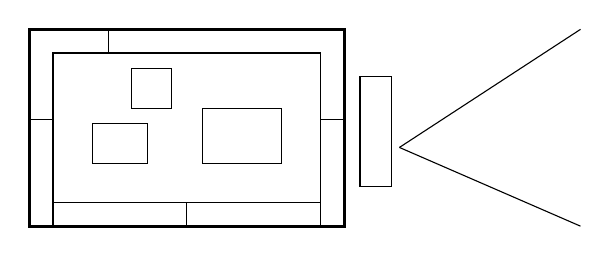
\begin{tikzpicture}	
	\scriptsize{
	\draw[fill=white,very thick,draw=black] (0,0) rectangle (4,2.5);
	\draw[fill=white!20,draw=black] (0.3,0.3) rectangle (3.7,2.2);
	
	\draw[fill=white,draw=black] (0.8,0.8) rectangle (1.5,1.3);		\node at (1.15,1.05) {};
	\draw[fill=white,draw=black] (2.2,.8) rectangle (3.2,1.5);		\node at (2.7,1.15) {};
	\draw[fill=white,draw=black] (1.3,1.5) rectangle (1.8,2.);		\node at (1.55,1.75) {};
	
	\draw[fill=white,draw=black] (4.2,.5) rectangle (4.6,1.9);		\node at (4.4,1.3) {};				
	
	\draw (4.7,1)--(7,2.5);
	\draw (4.7,1)--(7,0);
	\node at (6, 1.3) {};
	
	\node at (3,2.35) {};
	\node at (3.85,.6) {};
	\node at (3,.15) {};
	\node at (1,.15) {};
	\node at (0.15,.6) {};
	\node at (0.15,2) {};
	\node at (4.3,.15) {};
	
	\node at (3.4,.5) {};
	\node at (4.35,2.3) {};
	
	\draw (2,0)--(2,.3);
	\draw (1,2.2)--(1,2.5);	
	\draw (.3,.3)--(.3,0);
	\draw (0,1.35)--(.3,1.35);
	\draw (3.7,1.35)--(4,1.35);	
	\draw (3.7,.3)--(3.7,0);	
	}
\end{tikzpicture}
\end{center}
\caption{Separating disjoint polygons by an annulus.}	\label{fig:Cci2BciStar}
\end{figure}
\begin{lemma}\label{lma:Cci2Bci}
	There exists a -formula  with the following
	properties: \textup{(}i\textup{)}  entails  over ; \textup{(}ii\textup{)} if ,  are
	disjoint quasi-bounded polygons, then there exist
	polygons  such that .
\end{lemma}
\begin{proof}
Let  be the formula
	
	where  is the formula given in
	Lemma~\ref{lma:Cci2BciStar}. Property ({\em i}) is then immediate. For
	Property ({\em ii}), it is routine to show that there exist  polygons , 
	such that  and  is connected for ; let ,  be chosen analogously. Then for all  () and  () we have  and, by Lemma~\ref{lma:Newman},  connected. By Lemma~\ref{lma:Cci2BciStar}, let
	 be such that .
\end{proof}
We are now ready to prove:
\begin{swetheorem}{Theorem~\ref{theo:inftyBci}}
There is a -formula satisfiable over , but only by
regions with infinitely many components.
\end{swetheorem}
\begin{proof}
We first write a -formula,  with the required
properties, and then show that all occurrences of  can be
eliminated.  Note that  is not the same as the formula
 constructed for the proof of
Corollary~\ref{cor:inftyCci}.

Let , , , , , ,  and  
(, ) be variables. The constraints

are evidently satisfied by the arrangement of Fig.~\ref{fig:InfBci}.
\begin{figure}[h]
\begin{tikzpicture}[scale=1,
		c0/.style={fill=gray!5},
		c1/.style={fill=gray!5},
		c2/.style={fill=gray!25},
		c3/.style={fill=gray!25}
	]
		\scriptsize{
		\newcounter{md}\newcounter{mdf} \newcounter {mdd}
		\coordinate (H) at (0,5);\coordinate (P) at (0,0);
		\coordinate (Q) at (H);
		\coordinate (start) at (0,1.5);\coordinate (start') at ();\coordinate (first) at (0,2.9);\coordinate (first') at ();\coordinate (second) at (0,4);\coordinate (second') at ();\coordinate (end) at (H);\coordinate (end') at ();
		
		\coordinate (width) at (.8,0);
		
		\foreach \d in {0,...,35}
		{
			\pgfmathparse{.91^\d}			\let\factor=\pgfmathresult \pgfmathparse{2*mod(\d,2)-1}	\let\prt=\pgfmathresult
			\pgfmathsetcounter{mdf}{mod(\d,4)}
			\pgfmathsetcounter{md}{mod(\d,2)}
			\pgfmathsetcounter{mdd}{mod(\d/2,2)}
			
			\coordinate (Pm) at ();
			\coordinate (Qm) at ();
			\foreach \a/\ind in {-90/0,90/} {
				\coordinate (Pm') at ();
				\coordinate (Qm') at ();
				\coordinate (P\ind) at ();
				\coordinate (Q\ind) at ();
			}
			\draw[c\themdf] (P0)--(Q0)--(Q)--(P)--cycle;			
			
			\draw () 
				--();
			\draw ()
				--();			
			
			\coordinate (start) at ();\coordinate (start') at ();
			\coordinate (first) at ();\coordinate (first') at ();			
			\coordinate (second) at ();\coordinate (second') at ();
			\coordinate (end) at ();\coordinate (end') at ();
			
			\ifnum \d<6
				\ifnum \themd=0
					\node[rotate=81] at () {};
					\node[rotate=81] at () {};
					\node[rotate=81] at () {};
				\fi
				\ifnum \themd=1
					\node[rotate=-81] at () {};
					\node[rotate=-81] at () {};
					\node[rotate=-81] at () {};
				\fi
			\fi
		}
		}
\draw (-0.4,-0.4) rectangle (); 	\draw (0,0) rectangle ();
		\draw (0,0)--++(-.4,0);
		\draw (H)--++(0,.4);
		\draw ()--++(-.4,0);
		\draw ()--++(0,-.4);
		\draw () --++(.4,0);
		\draw () --++(.4,0);
		\node at (){};
		\node at (){};
		\node at (0,-.2){};
		\node at (){};
		\node at (){};
		\node at (3.8,-.2){};
		
	\end{tikzpicture}
\caption{A tuple of regions satisfying
  {\eqref{eq:BciInf1}--\eqref{eq:BciInf4}}: the pattern of components of the
   and  repeats forever.}
\label{fig:InfBci}
\end{figure}

Let  be the conjunction of~\eqref{eq:BciInf1}--\eqref{eq:BciInf4}
as well as all conjuncts

where  and  are any two distinct regions depicted on Fig.~\ref{fig:InfBci}. 
Note that the regions  and  have infinitely 
many  connected components. We will now show that this is true for every satisfying 
tuple of . 

By \eqref{eq:BciInf1}, we can use Lemma~\ref{lma:FrameLemmaInt} to construct 
a Jordan curve  whose segments 
are Jordan arcs lying in the respective sets , , 
, , , .
Further, let ,  and 
 (Fig.~\ref{subfig:BciFrame}). Note that all points in
,  and  that are on  are on ,  and , 
respectively. Let , and let . 
By \eqref{eq:BciInf2} and Lemma~\ref{lma:StackLemmai} 
we can connect  to  by a Jordan arc  
whose segments lie in the respective sets , 
 and  (Fig.~\ref{subfig:BciBeta0}). 
Let  be the last point on  that is on  and let  
be the final segment of  starting at . Similarly, let  
be the first point on  that is on  and let 
be the initial segment of  ending at . Hence, the arc  divides one of the regions bounded by  into two 
sub-regions. We denote the sub-region whose boundary is disjoint from  by , and 
the other sub-region we denote by . 
Let .
\begin{figure}[h]\begin{center}
\scriptsize{
	\subfloat[The arcs ,  and .]{
	\begin{tikzpicture}
		\clip (-.5,-.5) rectangle (3.5,2.5);
		\draw (0,0)rectangle(3,2);
		\fill (0,2) circle(1pt) node[above left]{};
		\fill (0,0) circle(1pt) node[below left]{};
		\fill (3,1) circle(1pt) node[right]{};		
		\draw (0,.75)  node[left]{};		
		\draw (1.5,2)  node[above]{};
		\draw (1.5,0)  node[below]{};
	\end{tikzpicture}\label{subfig:BciFrame}}
	\subfloat[The regions  and .]{
	\begin{tikzpicture}
		\clip (-.5,-.5) rectangle (3.5,2.5);
		\draw (0,0)rectangle(3,2);
		\foreach \x in {(0,2),(0,0),(3,1)} \fill \x circle(1pt);
		
		\fill (0,1.5) circle(1pt);
		\draw (0,1) circle(1pt) coordinate (o0') node[left]{};
		\draw(0,0.3) circle(1pt) coordinate (o0) node[left]{};
		\draw[densely dotted,decorate,decoration=snake] (o0') -- (o0);
		
		\draw (1.5,2) circle(1pt) coordinate(qs) node[above]{};
		\draw (1,2) circle(1pt) coordinate (q0) node[above]{};
		\draw[densely dotted,decorate,decoration=snake](q0)--(qs);

		\fill (o0)--() circle(1pt) node[midway,below right]{}--
					() circle(1pt) node[midway,below right]{}--
					(q0) node[midway,below right]{};
		\draw (o0)--(q0);
		\node at (.35,1.6){};
		\node at (2.25,1){};
	\end{tikzpicture}\label{subfig:BciBeta0}}\\
	\newcommand{\BciEstablishRegionsViUi}[1]{
	\begin{tikzpicture}
		\clip (-.5,-.5) rectangle (3.5,2.5);
\draw (0,0)rectangle(3,2);
		\foreach \x in {(0,2),(0,0),(3,1)} \fill \x circle(1pt);
\draw (0,.5) coordinate (p) circle(1pt)--(1.5,2) circle(1pt) coordinate(q);
		\node at (.35,1.75){};		
		\foreach \x in {0.2,0.9} \fill () circle(1pt);
\draw () circle(1pt) coordinate (e0') node[above left ]{};
		\draw () circle(1pt) coordinate (e0) node[above left]{};
		\draw[densely dotted,decorate,decoration=snake] (e0') --(e0);
		\draw (2,0) circle(1pt) coordinate(qs) node[below]{};
		\draw () circle(1pt) coordinate (p0) node[below]{}--(e0);
		\draw[densely dotted, decorate,decoration=snake] (p0)--(qs);
		\foreach \x in {0.3,0.7} \fill () circle(1pt);
		\node[right] at () {};
		\node[right] at () {};
		\node[right] at () {};
		\node at (.5,.4){};
		\node at (2.25,1){};
	\end{tikzpicture}\label{subfig:BciAlpha#1}}
	\subfloat[The regions  and .]{
	\BciEstablishRegionsViUi{0}}
	\subfloat[The regions redrawn.]{\label{subfig:BciRedrawn}
	\begin{tikzpicture}		
		\clip (-.5,-.5) rectangle (3.5,2.5);
\draw[densely dashed] (0,-.2) -- (0,2.2)--++(1.5,0)--++(0,-.2) coordinate(q0) node[above right]{};
		\draw[densely dashed] (0,-.2) --++(1.5,0)--++(0,.2)  coordinate (p0) node[below right]{};
		\foreach \x in {(0,2.2),(0,-.2),(3,1)} \fill \x circle(1pt);
		\foreach \x in {(p0),(q0)} \draw \x circle(1pt);
\coordinate (p) at (.75,2);
		\draw (.75,0) coordinate(q) rectangle (3,2);
		\foreach \x in {0,.55,1} \fill() circle(1pt);
		\draw[densely dashed] (0,1.25) coordinate(o0) node[left]{}--++(.75,0) coordinate(e0) node[right]{};
		\foreach \x in  {(o0),(e0)} \draw \x  circle(1pt);
		
		\node at (.35,1.75){};
		\node at (.35,.5){};
		\node at (1.1,.45){};
		\node at (2,1){};
		\draw[densely dotted, latex-latex,rounded corners=1pt] ()--
			(2.9,1.9) node[below left]{}--(2.9,1.1);
		\draw[densely dotted, latex-latex,rounded corners=2pt] ()--
			(2.9,.1) node[above left]{}--(2.9,.9);
	\end{tikzpicture}}\\
	\subfloat[The regions  and .]{\label{subfig:BciBeta1}
	\begin{tikzpicture}		
		\clip (-.5,-.5) rectangle (3.5,2.5);
\draw[densely dashed] (0,-.2) -- (0,1.75) coordinate(o0)--++(.75,0) coordinate (e0);
		\draw[densely dashed] (0,-.2) --++(1.5,0)--++(0,.2)  coordinate (p0);
		\foreach \x in {(0,-.2),(3,1)} \fill \x circle(1pt);
		\foreach \x in {(p0),(o0),(e0)} \draw \x circle(1pt);
\coordinate (p) at (.75,2);
		\draw (.75,0) coordinate(q) rectangle (3,2);
		\foreach \x in {0,.25,1} \fill() circle(1pt);
		
		\draw (.75,1.25) circle(1pt) coordinate (o1') node[left]{};
		\draw(.75,0.35) circle(1pt) coordinate (o1) node[right]{};
		\draw[densely dotted,decorate,decoration=snake] (o1') -- (o1);
		
		\draw (2,2) circle(1pt) coordinate(qs) node[above]{};
		\draw (1.5,2) circle(1pt) coordinate (q1) node[above]{};
		\draw[densely dotted,decorate,decoration=snake](q1)--(qs);
		
		\draw (o1)--(q1);
		\foreach \x in {.2,.8} \fill() circle(1pt);
		\node[below right] at () {};
		
		\node at (.35,.75){};
		\node at (1.1,1.75){};
		\node at (2.3,1){};
		
		\draw[densely dotted, latex-latex,rounded corners=2pt] ()--
			(2.9,.1) node[above left]{}--(2.9,.9);
	\end{tikzpicture}}
	\subfloat[The regions  and .]{\BciEstablishRegionsViUi{1}
	}}
	\end{center} \caption{Establishing infinite sequences of arcs.}
	\label{fig:BciInfCmp}
	\end{figure}

We will now construct a cross-cut  in . 
Let  and . By \eqref{eq:BciInf3} 
and Lemma~\ref{lma:StackLemmai} we can connect  to  by a Jordan arc 
 whose segments lie in the respective 
sets ,  and  
(Fig.~\ref{subfig:BciAlpha0}).  Let  be the last point on  that is on 
 and let  be the final segment of  starting at .
Similarly, let  be the first point on  that is on  and let 
be the initial segment of  ending at . By the non-overlapping constraints, 
 does not intersect the boundaries of  and 
except at its endpoints, and hence it is a cross-cut in one of these regions. Moreover, that region has 
to be  since the boundary of  is disjoint from . So,  divides  into two sub-regions. We denote the sub-region whose boundary contains 
  by , and the other sub-region we denote by . Let 
  (Fig~\ref{subfig:BciRedrawn}). Note that 
 .
 
 We can now forget about the region , and start constructing a cross-cut 
  in . As before, let 
 be a Jordan arc connecting a point  to a point 
  such that its segments are contained in the respective sets 
 ,  and . As before, we choose 
  and  so that the Jordan arc
  with its endpoints removed is disjoint from the boundaries of 
  and . Hence  has to be a cross-cut in  or 
 ,  and since the boundary of  is disjoint from  it has to be a cross-cut in  
   (Fig.~\ref{subfig:BciBeta1}). So,  separates  
 into two regions  and  so that the boundary of  is disjoint from .
 Let . Now, we can ignore 
 the region , and reasoning as before we can construct a cross-cut 
  in  dividing it into two sub-regions  and . 
\begin{figure}[h]
\begin{tikzpicture}[scale=1,
		c0/.style={fill=gray!5},
		c1/.style={fill=gray!5},
		c2/.style={fill=gray!25},
		c3/.style={fill=gray!25}
	]
		\clip (-.5,.5) rectangle (8,4.5);
		\scriptsize{
\coordinate (H) at (0,5);\coordinate (P) at (0,0);
		\coordinate (Q) at (H);
		\coordinate (start) at (0,1.5);\coordinate (start') at ();\coordinate (first) at (0,2.9);\coordinate (first') at ();\coordinate (second) at (0,4);\coordinate (second') at ();\coordinate (end) at (H);\coordinate (end') at ();
		
		\coordinate (width) at (.8,0);
		
		\foreach \d in {0,...,35}
		{
			\pgfmathparse{.91^\d}			\let\factor=\pgfmathresult \pgfmathparse{2*mod(\d,2)-1}	\let\prt=\pgfmathresult
			\pgfmathsetcounter{mdf}{mod(\d,4)}
			\pgfmathsetcounter{md}{mod(\d,2)}
			\pgfmathsetcounter{mdd}{mod(\d/2,2)}
			
			\coordinate (Pm) at ();
			\coordinate (Qm) at ();
			\foreach \a/\ind in {-90/0,90/} {
				\coordinate (Pm') at ();
				\coordinate (Qm') at ();
				\coordinate (P\ind) at ();
				\coordinate (Q\ind) at ();
			}
			\draw[c\themdf] (P0)--(Q0)--(Q)--(P)--cycle;			
			
			\draw () 
				--();
			\draw ()
				--();			
			
			\coordinate (start) at ();\coordinate (start') at ();
			\coordinate (first) at ();\coordinate (first') at ();			
			\coordinate (second) at ();\coordinate (second') at ();
			\coordinate (end) at ();\coordinate (end') at ();
			
			\ifnum \d<6
				\ifnum \themdd=0
					\ifnum \themd=0
						\node[rotate=81] at () {};
					\fi
					\ifnum \themd=1
						\node[rotate=-81] at () {};
					\fi
				\fi
			\fi
		}
		}
		\draw[thick] (4,1.6) ellipse (3.8 and 1.1);
\draw (-0.4,-0.4) rectangle (); 	\draw (0,0) rectangle ();
		\draw (0,0)--++(-.4,0);
		\draw (H)--++(0,.4);
		\draw ()--++(-.4,0);
		\draw ()--++(0,-.4);
		\draw () --++(.4,0);
		\draw () --++(.4,0);
		\node at (){};
		\node at (){};
		\node at (0,-.2){};
		\node at (){};
		\node at (){};
		\node at (3.8,-.2){};
	\end{tikzpicture}
\caption {Separating  from  by a Jordan curve.}
\label{fig:BciInftySep}
\end{figure}
 
 Evidently, this process continues forever. Now, note that by
 construction and \eqref{eq:BciInf5},  contains in its
 interior  together with the connected component 
 of  which contains . On the other hand,
  is disjoint from , and since , ,
  has to have infinitely many connected components.

So far we know that the -formula  forces
infinitely many components.  Now we replace every conjunct in
 of the form  by ,
where  are fresh variables each time. The resulting formula
entails , so we only have to show that it is still
satisfiable. By Lemma~\ref{lma:Cci2BciStar} (\emph{ii}), it suffices
to separate by Jordan curves every two regions on
Fig.~\ref{fig:InfBci} that are required to be disjoint. It is shown on
Fig.~\ref{fig:BciInftySep} that there exists a curve which separates
the regions  and . All other non-contact constraints
are treated analogously.
\end{proof}

\section{Undecidability of \cBc{} and \cBCc{} in the Euclidean plane}
\label{sec:UndecidabilityB}
In this section, we prove the undecidability of the problems
 and , for  any of
, ,  or . We begin with some technical
preliminaries, again employing the notation from the proof of
Theorem~\ref{theo:inftyBci}: if  is a Jordan arc, and , 
are points on  such that  occurs after , we denote by
 the segment of  from  to . For brevity of
exposition, we allow the case , treating  as a
(degenerate) Jordan arc.

Our first technical preliminary is to formalize our earlier observations
concerning the formula ,
defined by:

\begin{lemma}
\label{lma:stackLemma}
Let  be 3-regions satisfying
, for .  Then, for
every point  and every point , there exist points  and Jordan
arcs  such that\textup{:}
\begin{itemize}
\item[\textup{(}i\textup{)}]
 is a Jordan arc from  to
\textup{; }
\item[\textup{(}ii\textup{)}] for all  \textup{(}\textup{)}, \textup{;} and 
\item[\textup{(}iii\textup{)}]
for all  \textup{(}\textup{)}, .
\end{itemize}
\end{lemma}
\begin{proof}
Since  is a
connected subset of , let  be a Jordan arc connecting
 to  in . Since  is disjoint from all the 
except , let  be the first point of  lying in
, so , i.e., the arc  is either included in
, or is an end-cut of . (We do not rule out .) Similarly, let  be a Jordan arc connecting  to
 in , and let  be the last point of 
lying on . If , then set ,
, and .  so that the
endpoints of  are  and .  Otherwise, we have .  We can now construct an arc  from  to a point  on
, such that  intersects
 and  only at its endpoints,
 and  (upper diagram in Fig.~\ref{fig:stackLemma}). Let
, and let .

Since  contains a point , we may
iterate this procedure, obtaining . We remark that  and 
have a single point of contact by construction, while  and
 () are disjoint by the constraint .  Finally, we let  (lower diagram in
Fig.~\ref{fig:stackLemma}).
\end{proof}
\begin{figure}
\begin{center}
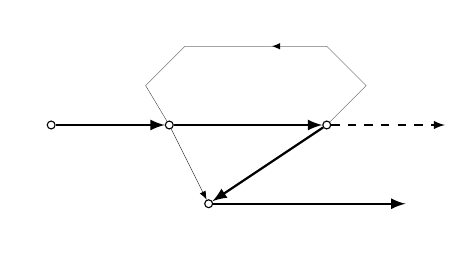
\begin{tikzpicture}[>=latex, point/.style={circle,draw=black,minimum size=1mm,inner sep=0pt}]
						
\node[point,label=left:{\small }] (P0) at (-0.5,0) {};
    \node[point,label=above right:{\small }] (Q1) at (1,0) {};
    \node[point,label=below left:{\small }] (Q1') at (1.5,-1) {};
    \node[point,label=above:{\small }] (P1) at (3,0) {};
    \draw[->,thick] (P0) to node[above] {\footnotesize } (Q1);
    \draw[->,thick] (Q1) to node[below] {\footnotesize } (P1);
    \draw[->,dashed] (P1) to node[above] {\footnotesize } (4.5,0);

	\draw[->,ultra thin] (P1) -- ++(.5,0.5) --++(-.5,.5)  -- (2.3,1);
	\draw[ultra thin] (2.3,1) to node[above, very near start]{\footnotesize } (1.2,1) -- ++(-.5,-0.5) -- (Q1);
    \draw[->,ultra thin] (Q1) to node[below,near start]{\footnotesize } (Q1');
	\draw[->,thick] (P1) to node[below,near start]{\footnotesize } (Q1');
	
	\draw[->,thick] (Q1') to node[below] {\footnotesize } (4,-1);
\end{tikzpicture}
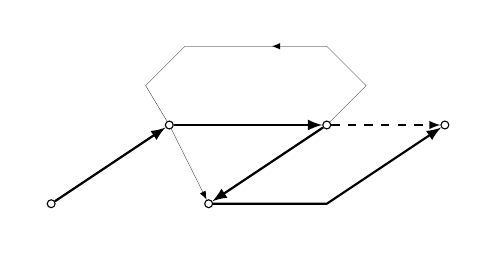
\begin{tikzpicture}[>=latex, point/.style={circle,draw=black,minimum size=1mm,inner sep=0pt}]
    \node[point,label=left:{\small }] (Qn2) at (6.5,-1) {};
    \node[point,label=above right:{\small }] (Qn1) at (8,0) {};
    \node[point,label=below left:{\small }] (Qn1') at (8.5,-1) {};
    \node[point,label=above:{\small }] (Pn1) at (10,0) {};
    \node[point,label=above:{\small }] (Pn) at (11.5,0) {};
    \draw[->,thick] (Qn2) to node[above] {\footnotesize } (Qn1);
    \draw[->,thick] (Qn1) to node[below] {\footnotesize } (Pn1);
    \draw[->,dashed] (Pn1) to node[above] {\footnotesize } (Pn);

	\draw[->,ultra thin] (Pn1) -- ++(.5,0.5) --++(-.5,.5)  -- (9.3,1);
	\draw[ultra thin] (9.3,1) to node[above, very near start]{\footnotesize } (8.2,1) -- ++(-.5,-0.5) -- (Qn1);
    \draw[->,ultra thin] (Qn1) to node[below,near start]{\footnotesize } (Qn1');
	\draw[->,thick] (Pn1) to node[below,near start]{\footnotesize } (Qn1');
	
	\draw[->,thick] (Qn1') to node[below] {\footnotesize } (10,-1) to (Pn);
\end{tikzpicture}
\end{center}
\caption{Proof of Lemma~\ref{lma:stackLemma}.}\label{fig:stackLemma}
\end{figure}

In fact, we can add a `switch'  to the formula , in the following sense.  If  is a region
variable, consider the formula 

where  denotes the 3-region . The first conjunct of
 ensures that any component
of  is either included in  or included in
. The second conjunct then has the same effect as
 for those components of
 included in . That is, if , we can find an arc  starting at , with the properties of
Lemma~\ref{lma:stackLemma}.  However, if , no such arc need exist.  Thus,  functions so as to
`de-activate' the formula 
for any component of  included in it.

As a further application of Lemma~\ref{lma:stackLemma}, consider the
formula  given by:

This formula allows us to construct Jordan curves in the plane, in
the following sense:
\begin{lemma}
\label{lma:FrameLemma}
Let , and suppose .  Then there exist Jordan arcs , \ldots,
 such that  is a Jordan
curve, and , for all , .
\end{lemma}
\begin{proof}
By , let
 be Jordan arcs in the respective
regions  such that, 
 is a Jordan arc connecting 
a point  to a 
point  (see 
Fig.~\ref{fig:FrameLemma}). Because  is a 
connected subset of the interior of , let  
be an arc connecting  and . Note that  does not intersect 
, for . Let  be the last point on  that 
is on  (possibly ), and  be the first point on  
that is on  (possibly ). Let  be the final segment of 
 starting at . Let , for .
Let  be the initial segment of  ending at .
Finally, take  to be the segment of  between  and .
Evidently, the arcs , , are as required.
\end{proof}
\begin{figure}[h]
\begin{center}
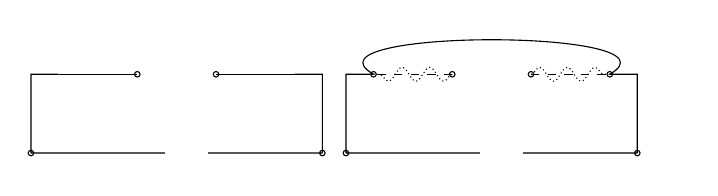
\begin{tikzpicture}
	\scriptsize{
		\draw (.5,1) circle(1pt) node[below]{};			
		\draw (.5,1) -- (1.5,1);
		\draw (1.5,1)--(1.85,1) --++(0,-1) node[left,near start]{} circle(1pt)
			--++(-1.45,0) node[midway,below]{}node[left]{};
		
		\draw (-.5,1) circle(1pt) node[below]{};
		\draw (-.5,1) -- (-1.5,1);
		\draw (-1.5,1)--(-1.85,1) --++(0,-1) node[right,near start]{} circle(1pt)
			--++(1.7,0) node[midway,below]{};
		
		\begin{scope}[xshift=4cm]
			\draw (.5,1) circle(1pt) node[below]{};
			\draw (1.5,1) circle(1pt) node[below]{};
			\draw[decorate,decoration=snake,densely dotted] (.5,1) -- (1.5,1);
			\draw[dashed] (.5,1) -- (1.5,1);
			\draw (1.5,1)--(1.85,1) --++(0,-1) node[left,midway]{} circle(1pt)
				--++(-1.45,0) node[midway,below]{}node[left]{};
			
			\draw (-.5,1) circle(1pt) node[below]{};
			\draw (-1.5,1) circle(1pt) node[below]{};
			\draw[decorate,decoration=snake,densely dotted] (-.5,1) -- (-1.5,1);
			\draw[dashed] (-.5,1) -- (-1.5,1);
			\draw (-1.5,1)--(-1.85,1) --++(0,-1) node[right,midway]{} circle(1pt)
				--++(1.7,0) node[midway,below]{};
			
			\draw(1.5,1) to[out=30,in=150] (-1.5,1) node[midway,below]{};
		\end{scope}
	}
\end{tikzpicture}
\end{center}
\caption{Establishing a Jordan curve.}
\label{fig:FrameLemma}
\end{figure}


Our final technical preliminary is a simple device for labelling arcs
in diagrams.
\begin{lemma}
\label{lma:labelling}
\label{lma:labels}
Suppose , , \ldots,  are regions such that

and let  be a connected subset of . Then  is included in
exactly one of the , .
\end{lemma}
\begin{proof}
If  and  are non-empty, then 
and  partition  into
non-empty, non-intersecting sets, closed in .
\end{proof}
When~\eqref{eq:labelling} holds, we may think of the regions  as `labels' for any connected ---and,
in particular, for any Jordan arc . Hence, any
sequence  of such arcs encodes a word over
the alphabet .

\bigskip

The remainder of this section is given over to a proof of
\begin{swetheorem}{Theorem~\ref{theo:undecidable}}
For ,
 is r.e.-hard, and
 is r.e.-complete.
\end{swetheorem}

We have already established the upper bounds; we consider here only
the lower bounds, beginning with an outline of our proof strategy.
Let a PCP-instance  be given,
where  is a finite alphabet, and  a word-morphism ().  We call the elements of 
    {\em tiles}, and, for each tile , we call  the {\em
      lower word} of , and  the {\em upper word} of
    . Thus,  asks whether there is a sequence of tiles
    (repeats allowed) such that the concatenation of their upper words
    is the same as the concatenation of their lower words. We shall
    henceforth restrict all (upper and lower) words on tiles to be
    non-empty.  This restriction simplifies the encoding below, and
    does not affect the undecidability of the PCP.

We define a formula  consisting of a large conjunction of
-literals, which, for ease of understanding, we introduce in
groups. Whenever conjuncts are introduced, it can be readily checked
that---provided  is positive---they are satisfiable by elements
of . (Figs.~\ref{fig:concrete1} and~\ref{fig:concrete2}
depict {\em part} of a satisfying assignment; this drawing is
additionally useful as an aid to intuition throughout the course of
the proof.)  The main object of the proof is to show that, conversely,
if  is satisfied by any tuple in , then 
must be positive. Thus, the following are equivalent:
\begin{enumerate}
\item  is positive;
\item  is satisfiable over ;
\item  is satisfiable over .
\end{enumerate}
This establishes the r.e.-hardness of  and
 for ; we then extend the result to the
languages ,  and .

\begin{figure}
\resizebox{9cm}{!}{\begin{picture}(0,0)\includegraphics{concrete1.pstex}\end{picture}\setlength{\unitlength}{3947sp}\begingroup\makeatletter\ifx\SetFigFont\undefined \gdef\SetFigFont#1#2#3#4#5{\reset@font\fontsize{#1}{#2pt}\fontfamily{#3}\fontseries{#4}\fontshape{#5}\selectfont}\fi\endgroup \begin{picture}(10974,4824)(514,-4573)
\put(751,-1786){\makebox(0,0)[lb]{\smash{{\SetFigFont{17}{20.4}{\rmdefault}{\mddefault}{\updefault}{\color[rgb]{0,0,0}}}}}}
\put(10951,-811){\makebox(0,0)[lb]{\smash{{\SetFigFont{17}{20.4}{\rmdefault}{\mddefault}{\updefault}{\color[rgb]{0,0,0}}}}}}
\put(10951,-1486){\makebox(0,0)[lb]{\smash{{\SetFigFont{17}{20.4}{\rmdefault}{\mddefault}{\updefault}{\color[rgb]{0,0,0}}}}}}
\put(10951,-2236){\makebox(0,0)[lb]{\smash{{\SetFigFont{17}{20.4}{\rmdefault}{\mddefault}{\updefault}{\color[rgb]{0,0,0}}}}}}
\put(751,-2236){\makebox(0,0)[lb]{\smash{{\SetFigFont{17}{20.4}{\rmdefault}{\mddefault}{\updefault}{\color[rgb]{0,0,0}}}}}}
\put(751,-361){\makebox(0,0)[lb]{\smash{{\SetFigFont{17}{20.4}{\rmdefault}{\mddefault}{\updefault}{\color[rgb]{0,0,0}}}}}}
\put(751,-1036){\makebox(0,0)[lb]{\smash{{\SetFigFont{17}{20.4}{\rmdefault}{\mddefault}{\updefault}{\color[rgb]{0,0,0}}}}}}
\put(751,-1411){\makebox(0,0)[lb]{\smash{{\SetFigFont{17}{20.4}{\rmdefault}{\mddefault}{\updefault}{\color[rgb]{0,0,0}}}}}}
\put(751,-661){\makebox(0,0)[lb]{\smash{{\SetFigFont{17}{20.4}{\rmdefault}{\mddefault}{\updefault}{\color[rgb]{0,0,0}}}}}}
\put(751,-2686){\makebox(0,0)[lb]{\smash{{\SetFigFont{17}{20.4}{\rmdefault}{\mddefault}{\updefault}{\color[rgb]{0,0,0}}}}}}
\put(751,-2986){\makebox(0,0)[lb]{\smash{{\SetFigFont{17}{20.4}{\rmdefault}{\mddefault}{\updefault}{\color[rgb]{0,0,0}}}}}}
\put(751,-3361){\makebox(0,0)[lb]{\smash{{\SetFigFont{17}{20.4}{\rmdefault}{\mddefault}{\updefault}{\color[rgb]{0,0,0}}}}}}
\put(751,-3736){\makebox(0,0)[lb]{\smash{{\SetFigFont{17}{20.4}{\rmdefault}{\mddefault}{\updefault}{\color[rgb]{0,0,0}}}}}}
\put(10951,-3811){\makebox(0,0)[lb]{\smash{{\SetFigFont{17}{20.4}{\rmdefault}{\mddefault}{\updefault}{\color[rgb]{0,0,0}}}}}}
\put(10951,-2986){\makebox(0,0)[lb]{\smash{{\SetFigFont{17}{20.4}{\rmdefault}{\mddefault}{\updefault}{\color[rgb]{0,0,0}}}}}}
\put(751,-4111){\makebox(0,0)[lb]{\smash{{\SetFigFont{17}{20.4}{\rmdefault}{\mddefault}{\updefault}{\color[rgb]{0,0,0}}}}}}
\put(5776,-136){\makebox(0,0)[lb]{\smash{{\SetFigFont{17}{20.4}{\rmdefault}{\mddefault}{\updefault}{\color[rgb]{0,0,0}}}}}}
\put(5851,-4336){\makebox(0,0)[lb]{\smash{{\SetFigFont{17}{20.4}{\rmdefault}{\mddefault}{\updefault}{\color[rgb]{0,0,0}}}}}}
\put(1801,-2236){\makebox(0,0)[lb]{\smash{{\SetFigFont{17}{20.4}{\rmdefault}{\mddefault}{\updefault}{\color[rgb]{0,0,0}}}}}}
\put(2851,-2236){\makebox(0,0)[lb]{\smash{{\SetFigFont{17}{20.4}{\rmdefault}{\mddefault}{\updefault}{\color[rgb]{0,0,0}}}}}}
\put(5776,-2236){\makebox(0,0)[lb]{\smash{{\SetFigFont{17}{20.4}{\rmdefault}{\mddefault}{\updefault}{\color[rgb]{0,0,0}}}}}}
\put(8776,-2236){\makebox(0,0)[lb]{\smash{{\SetFigFont{17}{20.4}{\rmdefault}{\mddefault}{\updefault}{\color[rgb]{0,0,0}}}}}}
\put(9901,-2236){\makebox(0,0)[lb]{\smash{{\SetFigFont{17}{20.4}{\rmdefault}{\mddefault}{\updefault}{\color[rgb]{0,0,0}}}}}}
\put(8401,-1036){\makebox(0,0)[lb]{\smash{{\SetFigFont{17}{20.4}{\rmdefault}{\mddefault}{\updefault}{\color[rgb]{0,0,0}}}}}}
\put(3376,-1111){\makebox(0,0)[lb]{\smash{{\SetFigFont{17}{20.4}{\rmdefault}{\mddefault}{\updefault}{\color[rgb]{0,0,0}}}}}}
\end{picture} }
\caption{A tuple
of 3-regions satisfying~{\eqref{eq:PCPFrame}}--{\eqref{eq:PCPCord}}. The 3-regions
 and  are shown in dotted lines.}
\label{fig:concrete1}
\end{figure}
The proof proceeds in five stages.
\bigskip

\noindent
\textbf{Stage 1.} In the first stage, we define an assemblage of arcs
that will serve as a scaffolding for the ensuing construction.
Consider the arrangement of polygonal 3-regions depicted in
Fig.~\ref{fig:concrete1}, assigned to the 3-region variables
, ,

as indicated. 
It is easy to verify that this arrangement can be made to
satisfy the following formulas:

And trivially, the arrangement can be made to satisfy any formula

for which the corresponding 3-regions  and  are
drawn as not being in contact. (Remember,  is the outer-most shell
of the 3-region , and similarly for .)  Thus, for
example, \eqref{eq:pcp:C} includes , but not  of .

Now suppose , ,  is {\em any} collection
of 3-regions (not necessarily polygonal)
satisfying~\eqref{eq:PCPFrame}--\eqref{eq:pcp:C}.  By
Lemma~\ref{lma:FrameLemma} and~\eqref{eq:PCPFrame}, let  be Jordan arcs included in
the respective regions , such that

is a Jordan curve (note that  and  have opposite
directions). We select points  on  and
 on  (see Fig.~\ref{fig:arcs0}).
By~\eqref{eq:PCPCord:endpoints}, 
and . By Lemma~\ref{lma:stackLemma}
and~\eqref{eq:PCPCord}, let , , 
be Jordan arcs in the respective regions

such that  is a Jordan arc from
 to . Let  be the last point of
 lying on , and let  be the final
segment of , starting at .  Let  be the
first point of  lying on , and let  be
the initial segment of , ending at .
\begin{figure}
\resizebox{8.5cm}{!}{\begin{picture}(0,0)\includegraphics{arcs0.pstex}\end{picture}\setlength{\unitlength}{3947sp}\begingroup\makeatletter\ifx\SetFigFont\undefined \gdef\SetFigFont#1#2#3#4#5{\reset@font\fontsize{#1}{#2pt}\fontfamily{#3}\fontseries{#4}\fontshape{#5}\selectfont}\fi\endgroup \begin{picture}(9542,5172)(451,-4567)
\put(451,389){\makebox(0,0)[lb]{\smash{{\SetFigFont{17}{20.4}{\rmdefault}{\mddefault}{\updefault}{\color[rgb]{0,0,0}}}}}}
\put(4876, 14){\makebox(0,0)[lb]{\smash{{\SetFigFont{17}{20.4}{\rmdefault}{\mddefault}{\updefault}{\color[rgb]{0,0,0}}}}}}
\put(5026,-4486){\makebox(0,0)[lb]{\smash{{\SetFigFont{17}{20.4}{\rmdefault}{\mddefault}{\updefault}{\color[rgb]{0,0,0}}}}}}
\put(9226,-1486){\makebox(0,0)[lb]{\smash{{\SetFigFont{17}{20.4}{\rmdefault}{\mddefault}{\updefault}{\color[rgb]{0,0,0}}}}}}
\put(9301,-2386){\makebox(0,0)[lb]{\smash{{\SetFigFont{17}{20.4}{\rmdefault}{\mddefault}{\updefault}{\color[rgb]{0,0,0}}}}}}
\put(9901,-811){\makebox(0,0)[lb]{\smash{{\SetFigFont{17}{20.4}{\rmdefault}{\mddefault}{\updefault}{\color[rgb]{0,0,0}}}}}}
\put(9976,-1861){\makebox(0,0)[lb]{\smash{{\SetFigFont{17}{20.4}{\rmdefault}{\mddefault}{\updefault}{\color[rgb]{0,0,0}}}}}}
\put(9976,-3436){\makebox(0,0)[lb]{\smash{{\SetFigFont{17}{20.4}{\rmdefault}{\mddefault}{\updefault}{\color[rgb]{0,0,0}}}}}}
\put(1501,-3511){\makebox(0,0)[lb]{\smash{{\SetFigFont{17}{20.4}{\rmdefault}{\mddefault}{\updefault}{\color[rgb]{0,0,0}}}}}}
\put(1576,-886){\makebox(0,0)[lb]{\smash{{\SetFigFont{17}{20.4}{\rmdefault}{\mddefault}{\updefault}{\color[rgb]{0,0,0}}}}}}
\put(601,-3586){\makebox(0,0)[lb]{\smash{{\SetFigFont{17}{20.4}{\rmdefault}{\mddefault}{\updefault}{\color[rgb]{0,0,0}}}}}}
\put(1426,-2686){\makebox(0,0)[lb]{\smash{{\SetFigFont{17}{20.4}{\rmdefault}{\mddefault}{\updefault}{\color[rgb]{0,0,0}}}}}}
\put(826,-2086){\makebox(0,0)[lb]{\smash{{\SetFigFont{17}{20.4}{\rmdefault}{\mddefault}{\updefault}{\color[rgb]{0,0,0}}}}}}
\put(826,-2686){\makebox(0,0)[lb]{\smash{{\SetFigFont{17}{20.4}{\rmdefault}{\mddefault}{\updefault}{\color[rgb]{0,0,0}}}}}}
\put(1801,-1861){\makebox(0,0)[lb]{\smash{{\SetFigFont{17}{20.4}{\rmdefault}{\mddefault}{\updefault}{\color[rgb]{0,0,0}}}}}}
\put(5326,-1861){\makebox(0,0)[lb]{\smash{{\SetFigFont{17}{20.4}{\rmdefault}{\mddefault}{\updefault}{\color[rgb]{0,0,0}}}}}}
\put(8626,-1861){\makebox(0,0)[lb]{\smash{{\SetFigFont{17}{20.4}{\rmdefault}{\mddefault}{\updefault}{\color[rgb]{0,0,0}}}}}}
\put(3076,-3736){\makebox(0,0)[lb]{\smash{{\SetFigFont{17}{20.4}{\rmdefault}{\mddefault}{\updefault}{\color[rgb]{0,0,0}}}}}}
\put(3451,-661){\makebox(0,0)[lb]{\smash{{\SetFigFont{17}{20.4}{\rmdefault}{\mddefault}{\updefault}{\color[rgb]{0,0,0}}}}}}
\end{picture} }
\caption{The arcs  and .}
\label{fig:arcs0}
\end{figure}
By~\eqref{eq:pcp:C}, we see that the arc 
intersects  only in its endpoints, and is thus a chord of
, as shown in Fig.~\ref{fig:arcs0}.

A word is required concerning the generality of this diagram.  The
reader is to imagine the figure drawn on a {\em spherical} canvas, of
which the sheet of paper or computer screen in front of him is simply
a small part.  This sphere represents the plane with a `point' at
infinity, under the usual stereographic projection. We do not say
where this point at infinity is, other than that it never lies on a
drawn arc.  In this way, a diagram in which the spherical canvas is
divided into  cells represents  different configurations in the
plane---one for each of the cells in which the point at infinity may
be located. For example, Fig~.\ref{fig:arcs0} represents three
topologically distinct configurations in , and, as such, depicts
the arcs , ,
, ,  and points ,  in full
generality.  All diagrams in this proof are to be interpreted in this
way.  We stress that our `spherical diagrams' are simply a convenient
device for using one drawing to represent several possible
configurations in the Euclidean plane: in particular, we are
interested only in the satisfiability of of -formulas over
 and , not over the regular closed algebra of
any other space!  For ease of reference, we refer to the the two
rectangles in Fig~.\ref{fig:arcs0} as the `upper window' and `lower
window', it being understood that these are simply handy labels: in
particular, either of these `windows' (but not both) may be unbounded.

\bigskip

\noindent
\textbf{Stage 2.}  In this stage, we we construct two sequences of
arcs, ,  of indeterminate length , such that the members of the former sequence all lie in the lower
window. Here and in the sequel, we write  to denote  modulo
3.  Let , ,  and 
(, ) be 3-region variables, let  be
an ordinary region-variable, and consider the formulas

The arrangement of polygonal 3-regions depicted in
Fig.~\ref{fig:concrete2} (with  assigned appropriately) is one such
satisfying assignment.
\begin{figure}
\resizebox{9cm}{!}{\begin{picture}(0,0)\includegraphics{concrete2.pstex}\end{picture}\setlength{\unitlength}{3947sp}\begingroup\makeatletter\ifx\SetFigFont\undefined \gdef\SetFigFont#1#2#3#4#5{\reset@font\fontsize{#1}{#2pt}\fontfamily{#3}\fontseries{#4}\fontshape{#5}\selectfont}\fi\endgroup \begin{picture}(13854,6279)(334,-5953)
\put(4576,-3811){\makebox(0,0)[lb]{\smash{{\SetFigFont{17}{20.4}{\rmdefault}{\mddefault}{\updefault}{\color[rgb]{0,0,0}}}}}}
\put(4576,-4411){\makebox(0,0)[lb]{\smash{{\SetFigFont{17}{20.4}{\rmdefault}{\mddefault}{\updefault}{\color[rgb]{0,0,0}}}}}}
\put(4576,-5011){\makebox(0,0)[lb]{\smash{{\SetFigFont{17}{20.4}{\rmdefault}{\mddefault}{\updefault}{\color[rgb]{0,0,0}}}}}}
\put(2626,-2461){\makebox(0,0)[lb]{\smash{{\SetFigFont{17}{20.4}{\rmdefault}{\mddefault}{\updefault}{\color[rgb]{0,0,0}}}}}}
\put(2626,-1636){\makebox(0,0)[lb]{\smash{{\SetFigFont{17}{20.4}{\rmdefault}{\mddefault}{\updefault}{\color[rgb]{0,0,0}}}}}}
\put(2626,-736){\makebox(0,0)[lb]{\smash{{\SetFigFont{17}{20.4}{\rmdefault}{\mddefault}{\updefault}{\color[rgb]{0,0,0}}}}}}
\put(1951,-3136){\makebox(0,0)[lb]{\smash{{\SetFigFont{17}{20.4}{\rmdefault}{\mddefault}{\updefault}{\color[rgb]{0,0,0}}}}}}
\put(1351,-3136){\makebox(0,0)[lb]{\smash{{\SetFigFont{17}{20.4}{\rmdefault}{\mddefault}{\updefault}{\color[rgb]{0,0,0}}}}}}
\put(2626,-3136){\makebox(0,0)[lb]{\smash{{\SetFigFont{17}{20.4}{\rmdefault}{\mddefault}{\updefault}{\color[rgb]{0,0,0}}}}}}
\put(3301,-3136){\makebox(0,0)[lb]{\smash{{\SetFigFont{17}{20.4}{\rmdefault}{\mddefault}{\updefault}{\color[rgb]{0,0,0}}}}}}
\put(3901,-3136){\makebox(0,0)[lb]{\smash{{\SetFigFont{17}{20.4}{\rmdefault}{\mddefault}{\updefault}{\color[rgb]{0,0,0}}}}}}
\put(4576,-3136){\makebox(0,0)[lb]{\smash{{\SetFigFont{17}{20.4}{\rmdefault}{\mddefault}{\updefault}{\color[rgb]{0,0,0}}}}}}
\put(6526,-736){\makebox(0,0)[lb]{\smash{{\SetFigFont{17}{20.4}{\rmdefault}{\mddefault}{\updefault}{\color[rgb]{0,0,0}}}}}}
\put(6526,-1636){\makebox(0,0)[lb]{\smash{{\SetFigFont{17}{20.4}{\rmdefault}{\mddefault}{\updefault}{\color[rgb]{0,0,0}}}}}}
\put(6526,-2461){\makebox(0,0)[lb]{\smash{{\SetFigFont{17}{20.4}{\rmdefault}{\mddefault}{\updefault}{\color[rgb]{0,0,0}}}}}}
\put(8476,-3136){\makebox(0,0)[lb]{\smash{{\SetFigFont{17}{20.4}{\rmdefault}{\mddefault}{\updefault}{\color[rgb]{0,0,0}}}}}}
\put(8476,-3811){\makebox(0,0)[lb]{\smash{{\SetFigFont{17}{20.4}{\rmdefault}{\mddefault}{\updefault}{\color[rgb]{0,0,0}}}}}}
\put(8476,-4411){\makebox(0,0)[lb]{\smash{{\SetFigFont{17}{20.4}{\rmdefault}{\mddefault}{\updefault}{\color[rgb]{0,0,0}}}}}}
\put(8476,-5011){\makebox(0,0)[lb]{\smash{{\SetFigFont{17}{20.4}{\rmdefault}{\mddefault}{\updefault}{\color[rgb]{0,0,0}}}}}}
\put(5251,-3136){\makebox(0,0)[lb]{\smash{{\SetFigFont{17}{20.4}{\rmdefault}{\mddefault}{\updefault}{\color[rgb]{0,0,0}}}}}}
\put(5851,-3136){\makebox(0,0)[lb]{\smash{{\SetFigFont{17}{20.4}{\rmdefault}{\mddefault}{\updefault}{\color[rgb]{0,0,0}}}}}}
\put(6526,-3136){\makebox(0,0)[lb]{\smash{{\SetFigFont{17}{20.4}{\rmdefault}{\mddefault}{\updefault}{\color[rgb]{0,0,0}}}}}}
\put(7201,-3136){\makebox(0,0)[lb]{\smash{{\SetFigFont{17}{20.4}{\rmdefault}{\mddefault}{\updefault}{\color[rgb]{0,0,0}}}}}}
\put(7876,-3136){\makebox(0,0)[lb]{\smash{{\SetFigFont{17}{20.4}{\rmdefault}{\mddefault}{\updefault}{\color[rgb]{0,0,0}}}}}}
\put(10426,-736){\makebox(0,0)[lb]{\smash{{\SetFigFont{17}{20.4}{\rmdefault}{\mddefault}{\updefault}{\color[rgb]{0,0,0}}}}}}
\put(10426,-1636){\makebox(0,0)[lb]{\smash{{\SetFigFont{17}{20.4}{\rmdefault}{\mddefault}{\updefault}{\color[rgb]{0,0,0}}}}}}
\put(12376,-3136){\makebox(0,0)[lb]{\smash{{\SetFigFont{17}{20.4}{\rmdefault}{\mddefault}{\updefault}{\color[rgb]{0,0,0}}}}}}
\put(12376,-3811){\makebox(0,0)[lb]{\smash{{\SetFigFont{17}{20.4}{\rmdefault}{\mddefault}{\updefault}{\color[rgb]{0,0,0}}}}}}
\put(12376,-4411){\makebox(0,0)[lb]{\smash{{\SetFigFont{17}{20.4}{\rmdefault}{\mddefault}{\updefault}{\color[rgb]{0,0,0}}}}}}
\put(12376,-5011){\makebox(0,0)[lb]{\smash{{\SetFigFont{17}{20.4}{\rmdefault}{\mddefault}{\updefault}{\color[rgb]{0,0,0}}}}}}
\put(9076,-3136){\makebox(0,0)[lb]{\smash{{\SetFigFont{17}{20.4}{\rmdefault}{\mddefault}{\updefault}{\color[rgb]{0,0,0}}}}}}
\put(9751,-3136){\makebox(0,0)[lb]{\smash{{\SetFigFont{17}{20.4}{\rmdefault}{\mddefault}{\updefault}{\color[rgb]{0,0,0}}}}}}
\put(10426,-3136){\makebox(0,0)[lb]{\smash{{\SetFigFont{17}{20.4}{\rmdefault}{\mddefault}{\updefault}{\color[rgb]{0,0,0}}}}}}
\put(11176,-3136){\makebox(0,0)[lb]{\smash{{\SetFigFont{17}{20.4}{\rmdefault}{\mddefault}{\updefault}{\color[rgb]{0,0,0}}}}}}
\put(11701,-3136){\makebox(0,0)[lb]{\smash{{\SetFigFont{17}{20.4}{\rmdefault}{\mddefault}{\updefault}{\color[rgb]{0,0,0}}}}}}
\put(10426,-2461){\makebox(0,0)[lb]{\smash{{\SetFigFont{17}{20.4}{\rmdefault}{\mddefault}{\updefault}{\color[rgb]{0,0,0}}}}}}
\put(5776,-136){\makebox(0,0)[lb]{\smash{{\SetFigFont{17}{20.4}{\rmdefault}{\mddefault}{\updefault}{\color[rgb]{0,0,0}}}}}}
\put(676,-3136){\makebox(0,0)[lb]{\smash{{\SetFigFont{17}{20.4}{\rmdefault}{\mddefault}{\updefault}{\color[rgb]{0,0,0}}}}}}
\put(6001,-5686){\makebox(0,0)[lb]{\smash{{\SetFigFont{17}{20.4}{\rmdefault}{\mddefault}{\updefault}{\color[rgb]{0,0,0}}}}}}
\put(7951,-136){\makebox(0,0)[lb]{\smash{{\SetFigFont{17}{20.4}{\rmdefault}{\mddefault}{\updefault}{\color[rgb]{0,0,0}}}}}}
\put(8176,-5686){\makebox(0,0)[lb]{\smash{{\SetFigFont{17}{20.4}{\rmdefault}{\mddefault}{\updefault}{\color[rgb]{0,0,0}}}}}}
\put(13126,-1636){\makebox(0,0)[lb]{\smash{{\SetFigFont{17}{20.4}{\rmdefault}{\mddefault}{\updefault}{\color[rgb]{0,0,0}}}}}}
\end{picture} }
\caption{A tuple of 3-regions
  satisfying~{\eqref{eq:aSeq1}}--{\eqref{eq:aSeq:a}}.
   The arrangement
  of components of the  and  repeats
  an indeterminate number of times. The 3-regions ,
   and one component of  are shown in dotted lines.
The 3-regions , ,  and 
are as in {Fig~\ref{fig:concrete2}}, but not drawn to scale.}
\label{fig:concrete2}
\end{figure}
We stipulate that~\eqref{eq:pcp:C} applies now to all regions depicted
in either Fig~\ref{fig:concrete1} or Fig~\ref{fig:concrete2}. Again,
    these additional constraints are evidently satisfiable.

It will be convenient in this stage to rename the arcs  and
 as  and , respectively.  Thus,
 forms the bottom edge of the lower window, and  the
top edge of the upper window. Likewise, we rename  as
, forming part of the left-hand side of the lower
window. Let  be any point of ,  any
point of , and  any point of  (see
Fig.~\ref{fig:arcs0}).  By~\eqref{eq:aSeq1}, then, , , and .  Adding the constraint

further ensures that .  By
Lemma~\ref{lma:stackLemma} and~\eqref{eq:aSeq:b}, we may draw an arc
 from  to , with successive
segments , , \ldots, ,
 lying in the respective regions , , \dots, , ; further, we can
guarantee that  contains a point .  Denote the last point of  by
. Also, let  be the last point of 
lying on , and  the first point of
 lying on  Finally, let  be the
segment of  between  and ; and we
let  be the segment of  from  to
 followed by the final segment of  from .
(Fig.~\ref{subfig:arcs1}).  By repeatedly using the constraints
in~\eqref{eq:pcp:C}, it is easy to see that that  together
with the initial segment of  up to  form a chord of
. Adding the constraints

and taking into account the constraints in~\eqref{eq:pcp:C} ensures
that  and  lie in the same residual domain of ,
as shown.  The wiggly lines indicate that we do not care about the
exact positions of  or ; otherwise,
Fig.~\ref{subfig:arcs1}) is again completely general.
\begin{figure}
\begin{center}
\subfloat[The arc .]{
\label{subfig:arcs1}
\resizebox{8cm}{!}{\begin{picture}(0,0)\includegraphics{subArcs1.pstex}\end{picture}\setlength{\unitlength}{3947sp}\begingroup\makeatletter\ifx\SetFigFont\undefined \gdef\SetFigFont#1#2#3#4#5{\reset@font\fontsize{#1}{#2pt}\fontfamily{#3}\fontseries{#4}\fontshape{#5}\selectfont}\fi\endgroup \begin{picture}(9012,4428)(601,-3973)
\put(1876,-661){\makebox(0,0)[lb]{\smash{{\SetFigFont{17}{20.4}{\rmdefault}{\mddefault}{\updefault}{\color[rgb]{0,0,0}}}}}}
\put(4351,239){\makebox(0,0)[lb]{\smash{{\SetFigFont{17}{20.4}{\rmdefault}{\mddefault}{\updefault}{\color[rgb]{0,0,0}}}}}}
\put(3151,-211){\makebox(0,0)[lb]{\smash{{\SetFigFont{17}{20.4}{\rmdefault}{\mddefault}{\updefault}{\color[rgb]{0,0,0}}}}}}
\put(2626,-1636){\makebox(0,0)[lb]{\smash{{\SetFigFont{17}{20.4}{\rmdefault}{\mddefault}{\updefault}{\color[rgb]{0,0,0}}}}}}
\put(1576,-1336){\makebox(0,0)[lb]{\smash{{\SetFigFont{17}{20.4}{\rmdefault}{\mddefault}{\updefault}{\color[rgb]{0,0,0}}}}}}
\put(6376,-2011){\makebox(0,0)[lb]{\smash{{\SetFigFont{17}{20.4}{\rmdefault}{\mddefault}{\updefault}{\color[rgb]{0,0,0}}}}}}
\put(1801,-2611){\makebox(0,0)[lb]{\smash{{\SetFigFont{17}{20.4}{\rmdefault}{\mddefault}{\updefault}{\color[rgb]{0,0,0}}}}}}
\put(4951,-811){\makebox(0,0)[lb]{\smash{{\SetFigFont{17}{20.4}{\rmdefault}{\mddefault}{\updefault}{\color[rgb]{0,0,0}}}}}}
\put(601,-3436){\makebox(0,0)[lb]{\smash{{\SetFigFont{17}{20.4}{\rmdefault}{\mddefault}{\updefault}{\color[rgb]{0,0,0}}}}}}
\put(601,-3061){\makebox(0,0)[lb]{\smash{{\SetFigFont{17}{20.4}{\rmdefault}{\mddefault}{\updefault}{\color[rgb]{0,0,0}}}}}}
\end{picture} }}\\
\subfloat[The arc .]{
\label{subfig:arcs2}
\resizebox{8cm}{!}{\begin{picture}(0,0)\includegraphics{subArcs2.pstex}\end{picture}\setlength{\unitlength}{3947sp}\begingroup\makeatletter\ifx\SetFigFont\undefined \gdef\SetFigFont#1#2#3#4#5{\reset@font\fontsize{#1}{#2pt}\fontfamily{#3}\fontseries{#4}\fontshape{#5}\selectfont}\fi\endgroup \begin{picture}(9012,4797)(601,-4792)
\put(4951,-886){\makebox(0,0)[lb]{\smash{{\SetFigFont{17}{20.4}{\rmdefault}{\mddefault}{\updefault}{\color[rgb]{0,0,0}}}}}}
\put(1801,-436){\makebox(0,0)[lb]{\smash{{\SetFigFont{17}{20.4}{\rmdefault}{\mddefault}{\updefault}{\color[rgb]{0,0,0}}}}}}
\put(2626,-1711){\makebox(0,0)[lb]{\smash{{\SetFigFont{17}{20.4}{\rmdefault}{\mddefault}{\updefault}{\color[rgb]{0,0,0}}}}}}
\put(601,-2986){\makebox(0,0)[lb]{\smash{{\SetFigFont{17}{20.4}{\rmdefault}{\mddefault}{\updefault}{\color[rgb]{0,0,0}}}}}}
\put(1501,-2686){\makebox(0,0)[lb]{\smash{{\SetFigFont{17}{20.4}{\rmdefault}{\mddefault}{\updefault}{\color[rgb]{0,0,0}}}}}}
\put(3751,-4711){\makebox(0,0)[lb]{\smash{{\SetFigFont{17}{20.4}{\rmdefault}{\mddefault}{\updefault}{\color[rgb]{0,0,0}}}}}}
\put(3901,-3061){\makebox(0,0)[lb]{\smash{{\SetFigFont{17}{20.4}{\rmdefault}{\mddefault}{\updefault}{\color[rgb]{0,0,0}}}}}}
\put(2176,-3286){\makebox(0,0)[lb]{\smash{{\SetFigFont{17}{20.4}{\rmdefault}{\mddefault}{\updefault}{\color[rgb]{0,0,0}}}}}}
\put(5551,-3661){\makebox(0,0)[lb]{\smash{{\SetFigFont{17}{20.4}{\rmdefault}{\mddefault}{\updefault}{\color[rgb]{0,0,0}}}}}}
\put(1651,-1036){\makebox(0,0)[lb]{\smash{{\SetFigFont{17}{20.4}{\rmdefault}{\mddefault}{\updefault}{\color[rgb]{0,0,0}}}}}}
\put(3076,-3811){\makebox(0,0)[lb]{\smash{{\SetFigFont{17}{20.4}{\rmdefault}{\mddefault}{\updefault}{\color[rgb]{0,0,0}}}}}}
\put(4201,-4261){\makebox(0,0)[lb]{\smash{{\SetFigFont{17}{20.4}{\rmdefault}{\mddefault}{\updefault}{\color[rgb]{0,0,0}}}}}}
\put(3076,-3511){\makebox(0,0)[lb]{\smash{{\SetFigFont{17}{20.4}{\rmdefault}{\mddefault}{\updefault}{\color[rgb]{0,0,0}}}}}}
\put(2776,-3136){\makebox(0,0)[lb]{\smash{{\SetFigFont{17}{20.4}{\rmdefault}{\mddefault}{\updefault}{\color[rgb]{0,0,0}}}}}}
\put(1651,-3586){\makebox(0,0)[lb]{\smash{{\SetFigFont{17}{20.4}{\rmdefault}{\mddefault}{\updefault}{\color[rgb]{0,0,0}}}}}}
\put(3151,-211){\makebox(0,0)[lb]{\smash{{\SetFigFont{17}{20.4}{\rmdefault}{\mddefault}{\updefault}{\color[rgb]{0,0,0}}}}}}
\end{picture} }}\\
\subfloat[The arc .]{
\label{subfig:arcs3}
\resizebox{8cm}{!}{\begin{picture}(0,0)\includegraphics{subArcs3.pstex}\end{picture}\setlength{\unitlength}{3947sp}\begingroup\makeatletter\ifx\SetFigFont\undefined \gdef\SetFigFont#1#2#3#4#5{\reset@font\fontsize{#1}{#2pt}\fontfamily{#3}\fontseries{#4}\fontshape{#5}\selectfont}\fi\endgroup \begin{picture}(8467,4797)(1146,-4492)
\put(1801,-436){\makebox(0,0)[lb]{\smash{{\SetFigFont{17}{20.4}{\rmdefault}{\mddefault}{\updefault}{\color[rgb]{0,0,0}}}}}}
\put(2176,-3286){\makebox(0,0)[lb]{\smash{{\SetFigFont{17}{20.4}{\rmdefault}{\mddefault}{\updefault}{\color[rgb]{0,0,0}}}}}}
\put(2851,-4036){\makebox(0,0)[lb]{\smash{{\SetFigFont{17}{20.4}{\rmdefault}{\mddefault}{\updefault}{\color[rgb]{0,0,0}}}}}}
\put(4876,-1711){\makebox(0,0)[lb]{\smash{{\SetFigFont{17}{20.4}{\rmdefault}{\mddefault}{\updefault}{\color[rgb]{0,0,0}}}}}}
\put(4051,-736){\makebox(0,0)[lb]{\smash{{\SetFigFont{17}{20.4}{\rmdefault}{\mddefault}{\updefault}{\color[rgb]{0,0,0}}}}}}
\put(3676,-3211){\makebox(0,0)[lb]{\smash{{\SetFigFont{17}{20.4}{\rmdefault}{\mddefault}{\updefault}{\color[rgb]{0,0,0}}}}}}
\put(2851,-2761){\makebox(0,0)[lb]{\smash{{\SetFigFont{17}{20.4}{\rmdefault}{\mddefault}{\updefault}{\color[rgb]{0,0,0}}}}}}
\put(5326, 89){\makebox(0,0)[lb]{\smash{{\SetFigFont{17}{20.4}{\rmdefault}{\mddefault}{\updefault}{\color[rgb]{0,0,0}}}}}}
\put(1726,-3811){\makebox(0,0)[lb]{\smash{{\SetFigFont{17}{20.4}{\rmdefault}{\mddefault}{\updefault}{\color[rgb]{0,0,0}}}}}}
\put(3151,-1411){\makebox(0,0)[lb]{\smash{{\SetFigFont{17}{20.4}{\rmdefault}{\mddefault}{\updefault}{\color[rgb]{0,0,0}}}}}}
\put(4051,-3811){\makebox(0,0)[lb]{\smash{{\SetFigFont{17}{20.4}{\rmdefault}{\mddefault}{\updefault}{\color[rgb]{0,0,0}}}}}}
\put(4201,-2461){\makebox(0,0)[lb]{\smash{{\SetFigFont{17}{20.4}{\rmdefault}{\mddefault}{\updefault}{\color[rgb]{0,0,0}}}}}}
\put(5926,-4411){\makebox(0,0)[lb]{\smash{{\SetFigFont{17}{20.4}{\rmdefault}{\mddefault}{\updefault}{\color[rgb]{0,0,0}}}}}}
\put(6451,-811){\makebox(0,0)[lb]{\smash{{\SetFigFont{17}{20.4}{\rmdefault}{\mddefault}{\updefault}{\color[rgb]{0,0,0}}}}}}
\end{picture} }}\\
\subfloat[The arc .]{
\label{subfig:arcs4}
\resizebox{8cm}{!}{\begin{picture}(0,0)\includegraphics{subArcs4.pstex}\end{picture}\setlength{\unitlength}{3947sp}\begingroup\makeatletter\ifx\SetFigFont\undefined \gdef\SetFigFont#1#2#3#4#5{\reset@font\fontsize{#1}{#2pt}\fontfamily{#3}\fontseries{#4}\fontshape{#5}\selectfont}\fi\endgroup \begin{picture}(8424,4021)(1189,-4016)
\put(6451,-811){\makebox(0,0)[lb]{\smash{{\SetFigFont{17}{20.4}{\rmdefault}{\mddefault}{\updefault}{\color[rgb]{0,0,0}}}}}}
\put(4126,-436){\makebox(0,0)[lb]{\smash{{\SetFigFont{17}{20.4}{\rmdefault}{\mddefault}{\updefault}{\color[rgb]{0,0,0}}}}}}
\put(5401,-3811){\makebox(0,0)[lb]{\smash{{\SetFigFont{17}{20.4}{\rmdefault}{\mddefault}{\updefault}{\color[rgb]{0,0,0}}}}}}
\put(7201,-3736){\makebox(0,0)[lb]{\smash{{\SetFigFont{17}{20.4}{\rmdefault}{\mddefault}{\updefault}{\color[rgb]{0,0,0}}}}}}
\put(3151,-1336){\makebox(0,0)[lb]{\smash{{\SetFigFont{17}{20.4}{\rmdefault}{\mddefault}{\updefault}{\color[rgb]{0,0,0}}}}}}
\put(5626,-211){\makebox(0,0)[lb]{\smash{{\SetFigFont{17}{20.4}{\rmdefault}{\mddefault}{\updefault}{\color[rgb]{0,0,0}}}}}}
\put(4126,-3661){\makebox(0,0)[lb]{\smash{{\SetFigFont{17}{20.4}{\rmdefault}{\mddefault}{\updefault}{\color[rgb]{0,0,0}}}}}}
\put(1276,-2011){\makebox(0,0)[lb]{\smash{{\SetFigFont{17}{20.4}{\rmdefault}{\mddefault}{\updefault}{\color[rgb]{0,0,0}}}}}}
\put(4426,-3211){\makebox(0,0)[lb]{\smash{{\SetFigFont{17}{20.4}{\rmdefault}{\mddefault}{\updefault}{\color[rgb]{0,0,0}}}}}}
\put(4276,-1636){\makebox(0,0)[lb]{\smash{{\SetFigFont{17}{20.4}{\rmdefault}{\mddefault}{\updefault}{\color[rgb]{0,0,0}}}}}}
\put(6226,-2761){\makebox(0,0)[lb]{\smash{{\SetFigFont{17}{20.4}{\rmdefault}{\mddefault}{\updefault}{\color[rgb]{0,0,0}}}}}}
\put(5401,-3211){\makebox(0,0)[lb]{\smash{{\SetFigFont{17}{20.4}{\rmdefault}{\mddefault}{\updefault}{\color[rgb]{0,0,0}}}}}}
\put(5401,-3511){\makebox(0,0)[lb]{\smash{{\SetFigFont{17}{20.4}{\rmdefault}{\mddefault}{\updefault}{\color[rgb]{0,0,0}}}}}}
\end{picture} }}
\end{center}
\caption{Construction of the arcs  and }
\label{fig:arcsAlphaBeta}
\end{figure}
Note that  lies entirely in , and hence
certainly in the region


Recall that , and .  By Lemma~\ref{lma:stackLemma} and~\eqref{eq:aSeq:a}, we may draw an arc
 from  to , with successive
segments , , \ldots,
,  lying in the respective regions
, , \dots,  ;
further, we can guarantee that the segment lying in  contains
a point .  Denote the last
point of  by .  Also, let  be the last
point of  lying on , and  the
first point of  lying on .
From~\eqref{eq:pcp:C}, these points must be arranged as shown in
Fig.~\ref{subfig:arcs2}.  Let  be the segment of
 between  and .  Noting
that~\eqref{eq:pcp:C} entails

we can be sure that  lies entirely in the `lower' window,
whence  crosses the central chord, , at least once. Let
 be the first such point (measured along  from left to
right).  Finally, let  be the segment of 
between  and , followed by the final segment of
 from . Note that  lies entirely in
, and hence certainly in the region

We remark that, in Fig.~\ref{subfig:arcs2}, the arcs  and
 have been slightly re-drawn, for clarity.  The region marked
 may now be forgotten, and is suppressed in Figs.~\ref{subfig:arcs3}
and~\ref{subfig:arcs4}.

By construction, the point  lies in some component of
, and, from the presence of the `switching'
variable  in~\eqref{eq:aSeq:a}, that component is either included
in  or included in . Suppose the latter.  Then we can repeat
the above construction to obtain an arc  from
 to , with successive segments
, , \ldots, ,
 lying in the respective regions , , \dots, , ; further, we can
guarantee that  contains a point .  Denote the last point of  by
. Also, let  be the last point of 
lying on , and  the first point of
 lying on .  Again, we let  be the
segment of  between  and ; and we
let  be the segment of  from  to
, followed by the final segment of  from .
Note that  lies in the set . It is easy to see that 
must be drawn as shown in Fig.~\ref{subfig:arcs3}: in particular,
 cannot enter the interior of the region marked . For,
by construction,  can have only one point of contact with
, and the constraints~\eqref{eq:pcp:C} ensure that 
cannot intersect any other part of ; since  is
guaranteed to lie outside , we evidently have . This observation having been made,  may now be
forgotten.

Symmetrically, we construct the arc , and points ,
, , together with the arcs arcs  and
, as shown in Fig.~\ref{subfig:arcs4} (where the region
 has been suppressed and the region  slightly
re-drawn). Again, we know from~\eqref{eq:pcp:C} that 
lies entirely in the `lower' window, whence  must cross the
central chord, , at least once. Let  be the first such
point (measured along  from left to right).

This process continues, generating arcs  and , as
long as  contains a point . That we
eventually reach a value  for which no such point exists
follows from~\eqref{eq:pcp:C}. For the conjuncts  () together entail , for every
 such that  is defined; and these points cycle on 
through the regions ,  and . If there were
infinitely many , the  would have an accumulation point,
lying in all three regions, contradicting, say, .  The resulting sequence of arcs and points is
shown, schematically, in Fig.~\ref{fig:arcs2}.
\begin{figure}
\resizebox{8.5cm}{!}{\begin{picture}(0,0)\includegraphics{5-1-Graphics/arcs2.pstex}\end{picture}\setlength{\unitlength}{3947sp}\begingroup\makeatletter\ifx\SetFigFont\undefined \gdef\SetFigFont#1#2#3#4#5{\reset@font\fontsize{#1}{#2pt}\fontfamily{#3}\fontseries{#4}\fontshape{#5}\selectfont}\fi\endgroup \begin{picture}(8467,3624)(1146,-3973)
\put(1651,-3436){\makebox(0,0)[lb]{\smash{{\SetFigFont{17}{20.4}{\rmdefault}{\mddefault}{\updefault}{\color[rgb]{0,0,0}}}}}}
\put(1276,-1711){\makebox(0,0)[lb]{\smash{{\SetFigFont{17}{20.4}{\rmdefault}{\mddefault}{\updefault}{\color[rgb]{0,0,0}}}}}}
\put(2401,-1711){\makebox(0,0)[lb]{\smash{{\SetFigFont{17}{20.4}{\rmdefault}{\mddefault}{\updefault}{\color[rgb]{0,0,0}}}}}}
\put(3601,-1711){\makebox(0,0)[lb]{\smash{{\SetFigFont{17}{20.4}{\rmdefault}{\mddefault}{\updefault}{\color[rgb]{0,0,0}}}}}}
\put(2926,-3436){\makebox(0,0)[lb]{\smash{{\SetFigFont{17}{20.4}{\rmdefault}{\mddefault}{\updefault}{\color[rgb]{0,0,0}}}}}}
\put(4276,-3436){\makebox(0,0)[lb]{\smash{{\SetFigFont{17}{20.4}{\rmdefault}{\mddefault}{\updefault}{\color[rgb]{0,0,0}}}}}}
\put(7501,-3361){\makebox(0,0)[lb]{\smash{{\SetFigFont{17}{20.4}{\rmdefault}{\mddefault}{\updefault}{\color[rgb]{0,0,0}}}}}}
\put(6901,-1786){\makebox(0,0)[lb]{\smash{{\SetFigFont{17}{20.4}{\rmdefault}{\mddefault}{\updefault}{\color[rgb]{0,0,0}}}}}}
\end{picture} }
\caption{The sequences of arcs  and .}
\label{fig:arcs2}
\end{figure}

We finish this stage in the construction by `re-packaging' the arcs
 and , as illustrated in
Fig.~\ref{fig:arcs3}. Specifically,
for all  (), let  be the initial segment
of  up to the point  followed by the initial segment
of  up to the point ; and let  be the
final segment of  from the point :

The final
segment of  from the point  may be forgotten.
\begin{figure}
\resizebox{8cm}{!}{\begin{picture}(0,0)\includegraphics{arcs3.pstex}\end{picture}\setlength{\unitlength}{3947sp}\begingroup\makeatletter\ifx\SetFigFont\undefined \gdef\SetFigFont#1#2#3#4#5{\reset@font\fontsize{#1}{#2pt}\fontfamily{#3}\fontseries{#4}\fontshape{#5}\selectfont}\fi\endgroup \begin{picture}(8274,3297)(3439,-3892)
\put(8326,-2761){\makebox(0,0)[lb]{\smash{{\SetFigFont{17}{20.4}{\rmdefault}{\mddefault}{\updefault}{\color[rgb]{0,0,0}}}}}}
\put(10276,-2836){\makebox(0,0)[lb]{\smash{{\SetFigFont{17}{20.4}{\rmdefault}{\mddefault}{\updefault}{\color[rgb]{0,0,0}}}}}}
\put(9676,-2761){\makebox(0,0)[lb]{\smash{{\SetFigFont{17}{20.4}{\rmdefault}{\mddefault}{\updefault}{\color[rgb]{0,0,0}}}}}}
\put(9076,-1861){\makebox(0,0)[lb]{\smash{{\SetFigFont{17}{20.4}{\rmdefault}{\mddefault}{\updefault}{\color[rgb]{0,0,0}}}}}}
\put(9301,-811){\makebox(0,0)[lb]{\smash{{\SetFigFont{17}{20.4}{\rmdefault}{\mddefault}{\updefault}{\color[rgb]{0,0,0}}}}}}
\put(3526,-1936){\makebox(0,0)[lb]{\smash{{\SetFigFont{17}{20.4}{\rmdefault}{\mddefault}{\updefault}{\color[rgb]{0,0,0}}}}}}
\put(7951,-1936){\makebox(0,0)[lb]{\smash{{\SetFigFont{17}{20.4}{\rmdefault}{\mddefault}{\updefault}{\color[rgb]{0,0,0}}}}}}
\put(4651,-1861){\makebox(0,0)[lb]{\smash{{\SetFigFont{17}{20.4}{\rmdefault}{\mddefault}{\updefault}{\color[rgb]{0,0,0}}}}}}
\put(5926,-3811){\makebox(0,0)[lb]{\smash{{\SetFigFont{17}{20.4}{\rmdefault}{\mddefault}{\updefault}{\color[rgb]{0,0,0}}}}}}
\put(5251,-3361){\makebox(0,0)[lb]{\smash{{\SetFigFont{17}{20.4}{\rmdefault}{\mddefault}{\updefault}{\color[rgb]{0,0,0}}}}}}
\put(5776,-2761){\makebox(0,0)[lb]{\smash{{\SetFigFont{17}{20.4}{\rmdefault}{\mddefault}{\updefault}{\color[rgb]{0,0,0}}}}}}
\put(4951,-811){\makebox(0,0)[lb]{\smash{{\SetFigFont{17}{20.4}{\rmdefault}{\mddefault}{\updefault}{\color[rgb]{0,0,0}}}}}}
\put(4201,-3211){\makebox(0,0)[lb]{\smash{{\SetFigFont{17}{20.4}{\rmdefault}{\mddefault}{\updefault}{\color[rgb]{0,0,0}}}}}}
\put(5251,-2761){\makebox(0,0)[lb]{\smash{{\SetFigFont{17}{20.4}{\rmdefault}{\mddefault}{\updefault}{\color[rgb]{0,0,0}}}}}}
\put(9601,-3361){\makebox(0,0)[lb]{\smash{{\SetFigFont{17}{20.4}{\rmdefault}{\mddefault}{\updefault}{\color[rgb]{0,0,0}}}}}}
\end{picture} }
\caption{`Re-packaging' of  and  into  and
  : before and after.}
\label{fig:arcs3}
\end{figure}
Defining, for ,

the constraints~\eqref{eq:pcp:C} guarantee that, for ,

Observe that the arcs  are located entirely in the `lower
window', and that each arc  connects  to some point
, which in turn is connected to a point 
by an arc in .

\bigskip

\noindent
\textbf{Stage 3.}  We now repeat Stage~2 symmetrically, with the
`upper' and `lower' windows exchanged. Let ,
 be 3-region variables (with indices in the same
ranges as for , ). Let , ; and let

for . The constraints

then establish sequences of arcs , ,
() satisfying

for . The arcs  are located entirely in the
`upper window', and each arc  connects  to a point
, which in turn is connected to a point  by an arc in
the region

Our next task is to write constraints to ensure that , and
that, furthermore, each  (also each ) connects
 to , for . Let  be a new
region-variable, and write

Note that  does not appear in this constraint, which ensures that
the only arc depicted in Fig.~\ref{fig:arcs0} which  may intersect
is . Recalling that  and  contain
points  and , respectively, both lying in , the
constraints

ensure that  and  may be joined by an arc, say
, lying in , and also lying entirely in the upper
and lower windows, crossing  only in .  Without loss of
generality, we may assume that  contacts  and
 in just one point. Bearing in mind that the
constraints~\eqref{eq:pcp:C} force  and  to
cross  in its central section, , writing

for all  () and  () ensures that
 is (essentially) as shown in Fig.~\ref{fig:arcZeta}.
\begin{figure}
\resizebox{8.5cm}{!}{\begin{picture}(0,0)\includegraphics{arcZeta.pstex}\end{picture}\setlength{\unitlength}{3947sp}\begingroup\makeatletter\ifx\SetFigFont\undefined \gdef\SetFigFont#1#2#3#4#5{\reset@font\fontsize{#1}{#2pt}\fontfamily{#3}\fontseries{#4}\fontshape{#5}\selectfont}\fi\endgroup \begin{picture}(9624,3624)(1189,-3973)
\put(7576,-3511){\makebox(0,0)[lb]{\smash{{\SetFigFont{17}{20.4}{\rmdefault}{\mddefault}{\updefault}{\color[rgb]{0,0,0}}}}}}
\put(8251,-2611){\makebox(0,0)[lb]{\smash{{\SetFigFont{17}{20.4}{\rmdefault}{\mddefault}{\updefault}{\color[rgb]{0,0,0}}}}}}
\put(10051,-1486){\makebox(0,0)[lb]{\smash{{\SetFigFont{17}{20.4}{\rmdefault}{\mddefault}{\updefault}{\color[rgb]{0,0,0}}}}}}
\put(1726,-961){\makebox(0,0)[lb]{\smash{{\SetFigFont{17}{20.4}{\rmdefault}{\mddefault}{\updefault}{\color[rgb]{0,0,0}}}}}}
\put(3001,-961){\makebox(0,0)[lb]{\smash{{\SetFigFont{17}{20.4}{\rmdefault}{\mddefault}{\updefault}{\color[rgb]{0,0,0}}}}}}
\put(1651,-3511){\makebox(0,0)[lb]{\smash{{\SetFigFont{17}{20.4}{\rmdefault}{\mddefault}{\updefault}{\color[rgb]{0,0,0}}}}}}
\put(2926,-3511){\makebox(0,0)[lb]{\smash{{\SetFigFont{17}{20.4}{\rmdefault}{\mddefault}{\updefault}{\color[rgb]{0,0,0}}}}}}
\put(7426,-1711){\makebox(0,0)[lb]{\smash{{\SetFigFont{17}{20.4}{\rmdefault}{\mddefault}{\updefault}{\color[rgb]{0,0,0}}}}}}
\put(7951,-961){\makebox(0,0)[lb]{\smash{{\SetFigFont{17}{20.4}{\rmdefault}{\mddefault}{\updefault}{\color[rgb]{0,0,0}}}}}}
\put(9451,-1861){\makebox(0,0)[lb]{\smash{{\SetFigFont{17}{20.4}{\rmdefault}{\mddefault}{\updefault}{\color[rgb]{0,0,0}}}}}}
\put(3301,-1861){\makebox(0,0)[lb]{\smash{{\SetFigFont{17}{20.4}{\rmdefault}{\mddefault}{\updefault}{\color[rgb]{0,0,0}}}}}}
\end{picture} }
\caption{The arc .}
\label{fig:arcZeta}
\end{figure}
Now consider the arc . Recalling that  joins
 to the point  (on the upper edge of the upper window),
crossing , we see by inspection of Fig.~\ref{fig:arcZeta}
that~\eqref{eq:zeta} together with

for 
forces  to cross one of the arcs
 (); and the constraints

for , , , ensure that  modulo 3. We write the symmetric constraints

for , , , together with 

for .  Now suppose .  The arc  must connect  to the point  on the bottom
edge of the lower window, which is now impossible without 
crossing either  or ---both forbidden
by~\eqref{eq:abPrime}--\eqref{eq:bbPrime}.  Thus,  intersects
 if and only if . Symmetrically,  intersects
 if and only if .  And the reasoning can now be
repeated for , , ,  \ldots, leading
to the 1--1 correspondence depicted in
Fig.~\ref{fig:arcCorrespondence}.
\begin{figure}
\resizebox{8cm}{!}{\begin{picture}(0,0)\includegraphics{arcCorrespondence.pstex}\end{picture}\setlength{\unitlength}{3947sp}\begingroup\makeatletter\ifx\SetFigFont\undefined \gdef\SetFigFont#1#2#3#4#5{\reset@font\fontsize{#1}{#2pt}\fontfamily{#3}\fontseries{#4}\fontshape{#5}\selectfont}\fi\endgroup \begin{picture}(9624,3624)(1189,-3973)
\put(3901,-1786){\makebox(0,0)[lb]{\smash{{\SetFigFont{17}{20.4}{\rmdefault}{\mddefault}{\updefault}{\color[rgb]{0,0,0}}}}}}
\put(10276,-1936){\makebox(0,0)[lb]{\smash{{\SetFigFont{17}{20.4}{\rmdefault}{\mddefault}{\updefault}{\color[rgb]{0,0,0}}}}}}
\put(7651,-3436){\makebox(0,0)[lb]{\smash{{\SetFigFont{17}{20.4}{\rmdefault}{\mddefault}{\updefault}{\color[rgb]{0,0,0}}}}}}
\put(7351,-1936){\makebox(0,0)[lb]{\smash{{\SetFigFont{17}{20.4}{\rmdefault}{\mddefault}{\updefault}{\color[rgb]{0,0,0}}}}}}
\put(1501,-1786){\makebox(0,0)[lb]{\smash{{\SetFigFont{17}{20.4}{\rmdefault}{\mddefault}{\updefault}{\color[rgb]{0,0,0}}}}}}
\put(2701,-1786){\makebox(0,0)[lb]{\smash{{\SetFigFont{17}{20.4}{\rmdefault}{\mddefault}{\updefault}{\color[rgb]{0,0,0}}}}}}
\put(1576,-3361){\makebox(0,0)[lb]{\smash{{\SetFigFont{17}{20.4}{\rmdefault}{\mddefault}{\updefault}{\color[rgb]{0,0,0}}}}}}
\put(2851,-3361){\makebox(0,0)[lb]{\smash{{\SetFigFont{17}{20.4}{\rmdefault}{\mddefault}{\updefault}{\color[rgb]{0,0,0}}}}}}
\put(4051,-3361){\makebox(0,0)[lb]{\smash{{\SetFigFont{17}{20.4}{\rmdefault}{\mddefault}{\updefault}{\color[rgb]{0,0,0}}}}}}
\end{picture} }
\caption{The 1--1 correspondence between the  and the
   established by the  and the .}
\label{fig:arcCorrespondence}
\end{figure}
In particular, we are guaranteed that .

\bigskip

\noindent
\textbf{Stage 4.}  Recall the given PCP-instance, .  We think of  as a set of `tiles', and the
morphisms ,  as specifying, respectively, the `lower'
and `upper' strings of each tile.  In this stage, we shall `label' the arcs
, with elements of , thus
defining a word  over this alphabet. Using a slightly more
complicated labelling scheme, we shall label the arcs  so as to define a word  (of length ) over the
alphabet ; likewise we shall label the arcs 
so as to define another word  (of length ) over .

We begin with the . Consider the constraints

By Lemma~\ref{lma:labelling}, in any satisfying assignment over
, every arc  () is included in
(`labelled with') exactly one of the regions  or , so that
the sequence of arcs  defines a word , with .

Turning our attention now to the , let us write . For all  (), we
shall write  and ;
further, we denote  by  and  by
. (Thus, by assumption, the  and  are all
positive.)

Now let  (, ) and
 (, ) be fresh
region variables.  We think of  as standing for the th
letter in the word , and likewise think of  as
standing for the th letter in the word .  By
Lemma~\ref{lma:labelling}, we may write constraints ensuring that each
component of either ,  or ---and hence each of the arcs
---is `labelled with' one of the ,
in the by-now familiar sense.  Further, we can ensure that these
labels are organized into (contiguous) blocks, 
such that, in the th block, , the sequence of labels reads
, for some fixed  ().  This amounts to insisting that: ({\em i}) the very first arc,
, must be labelled with  for some ; ({\em ii})
if,  is labelled with , where  and , then the next arc, namely , must be labelled with
the next letter of , namely ; ({\em iii}) if
 () is labelled with the final letter of , then
the next arc must be labelled with the initial letter of some possibly
different word ; and ({\em iv})  must be
labelled with the final letter of some word. To do this we simply
write:

where ,  and .

Thus, within each block , the labels read , for some fixed ; we write  to denote the
common subscript .  The sequence of indices 
corresponding to the successive blocks thus defines a word .

Using corresponding formulas, we label the arcs  () with the alphabet , so that, in any satisfying assignment over
, every arc  () is labelled with
exactly one of the regions . Further, we can ensure that
these labels are organized into (say)  contiguous blocks,  such that in the th block, , the sequence of
labels reads , for some fixed
. Again, writing  for the common value of , the sequence
of of indices  corresponding to the successive
blocks defines a word .


\bigskip

\noindent
\textbf{Stage 5.}  The basic job of the foregoing stages was to define
the words  and .  In this
stage, we enforce the equations ,  and . That is: the PCP-instance  is positive.

We first add the constraints

Since  is in contact with  for all  (), the string  defined by the arcs 
must be identical to the string . But this is just to say that .
The equation  may be secured similarly.

It remains only to show that .  That is, we must show
that  and that, for all  (), . The techniques required have in fact already been encountered
in Stage~3.  We first introduce a new pair of variables, , ,
which we refer to as `block colours', and with which we label the arcs
 in the fashion of Lemma~\ref{lma:labelling}, using the
constraints:

We force all arcs in each block  to have a uniform block colour,
and we force the block colours to alternate by writing, for ,
,  and :

Thus, we may speak unambiguously of the colour ( or ) of a
block: if  is coloured , then  will be coloured ,
 coloured , and so on.  Using the the {\em same} variables
 and , we similarly establish a block structure  on the arcs . (Note that there is no need
for primed versions of  and .)

Now we can match up the blocks in a 1--1
fashion just as we matched up the individual arcs. Let ,
,  and  be new 3-regions
variables.  We may assume that every arc  contains some point
of . We wish to connect any such arc that
starts a block  (i.e. any  labelled by  for
some ) to the top edge of the upper window, with the connecting arc
depending on the block colour.  Setting  (), we can do this using the
constraints:

Specifically, the first arc in each block  () is
connected by an arc  to some point on the
upper edge of the upper window, where 
and .  Similarly, setting
 (), 
the constraints

ensure that the first arc in each block  () is connected by an arc  to some
point on the bottom edge of the lower window, where  and .
Furthermore, from the arrangement of the ,
 and  (Fig.~\ref{fig:arcZeta}) we can easily write
non-contact constraints
forcing each  to intersect one of the arcs  (), and each  to intersect one of the arcs
 ().

We now write the constraints

Thus, any  included in  must join some arc  in
a block with colour  to some arc  also in a block
with colour ; and similarly for the .
Adding

then ensures, via reasoning exactly similar to that employed in
Stage~3, that  connects the block  to the block ,
 connects  to , and so on; and similarly for the
 (as shown, schematically, in
Fig.~\ref{fig:blockCorrespondence}).  Thus, we have a 1--1
correspondence between the two sets of blocks, whence .
\begin{figure}
\resizebox{9cm}{!}{\begin{picture}(0,0)\includegraphics{blockCorrespondence.pstex}\end{picture}\setlength{\unitlength}{3947sp}\begingroup\makeatletter\ifx\SetFigFont\undefined \gdef\SetFigFont#1#2#3#4#5{\reset@font\fontsize{#1}{#2pt}\fontfamily{#3}\fontseries{#4}\fontshape{#5}\selectfont}\fi\endgroup \begin{picture}(9634,3624)(1179,-3973)
\put(7801,-2611){\makebox(0,0)[lb]{\smash{{\SetFigFont{17}{20.4}{\rmdefault}{\mddefault}{\updefault}{\color[rgb]{0,0,0}}}}}}
\put(4051,-2611){\makebox(0,0)[lb]{\smash{{\SetFigFont{17}{20.4}{\rmdefault}{\mddefault}{\updefault}{\color[rgb]{0,0,0}}}}}}
\put(6601,-2611){\makebox(0,0)[lb]{\smash{{\SetFigFont{17}{20.4}{\rmdefault}{\mddefault}{\updefault}{\color[rgb]{0,0,0}}}}}}
\put(1351,-2611){\makebox(0,0)[lb]{\smash{{\SetFigFont{17}{20.4}{\rmdefault}{\mddefault}{\updefault}{\color[rgb]{0,0,0}}}}}}
\put(2101,-2611){\makebox(0,0)[lb]{\smash{{\SetFigFont{17}{20.4}{\rmdefault}{\mddefault}{\updefault}{\color[rgb]{0,0,0}}}}}}
\put(3001,-2611){\makebox(0,0)[lb]{\smash{{\SetFigFont{17}{20.4}{\rmdefault}{\mddefault}{\updefault}{\color[rgb]{0,0,0}}}}}}
\put(1801,-886){\makebox(0,0)[lb]{\smash{{\SetFigFont{17}{20.4}{\rmdefault}{\mddefault}{\updefault}{\color[rgb]{0,0,0}}}}}}
\put(4426,-3511){\makebox(0,0)[lb]{\smash{{\SetFigFont{17}{20.4}{\rmdefault}{\mddefault}{\updefault}{\color[rgb]{0,0,0}}}}}}
\put(2776,-886){\makebox(0,0)[lb]{\smash{{\SetFigFont{17}{20.4}{\rmdefault}{\mddefault}{\updefault}{\color[rgb]{0,0,0}}}}}}
\put(2176,-3511){\makebox(0,0)[lb]{\smash{{\SetFigFont{17}{20.4}{\rmdefault}{\mddefault}{\updefault}{\color[rgb]{0,0,0}}}}}}
\put(8026,-886){\makebox(0,0)[lb]{\smash{{\SetFigFont{17}{20.4}{\rmdefault}{\mddefault}{\updefault}{\color[rgb]{0,0,0}}}}}}
\put(9751,-1111){\makebox(0,0)[lb]{\smash{{\SetFigFont{17}{20.4}{\rmdefault}{\mddefault}{\updefault}{\color[rgb]{0,0,0}}}}}}
\put(7651,-3511){\makebox(0,0)[lb]{\smash{{\SetFigFont{17}{20.4}{\rmdefault}{\mddefault}{\updefault}{\color[rgb]{0,0,0}}}}}}
\end{picture} }
\caption{The 1--1 correspondence between the  and the
   established by the  and the .}
\label{fig:blockCorrespondence}
\end{figure}

Finally, we let  be
new regions variables labelling the components of  and of ,
and hence the arcs :

for . Adding the constraints

where ,  and , instantly ensures that the sequences of tile indices  and  are identical. In other words,
.  This completes the proof that  is a positive
instance of the PCP.

We have established the r.e.-hardness of  and
. We must now extend these results to the
other languages considered here. We deal with the languages 
and  as in Sec.~\ref{sec:sensitivity}. Let  be
the  formula obtained by replacing all of occurrences of 
in  with . Since all occurrences of  in 
are positive,  entails . On the other
hand, the connected regions satisfying  are also
interior-connected, and thus satisfy  as well.

For the language , observe that, as in Sec.~\ref{sec:sensitivity},  
all conjuncts of  featuring the predicate  are {\em negative}. 
(Remember that there are additional such literals
implicit in the use of 3-region variables; but let us ignore these for
the moment.) Recall from Sec.~\ref{sec:sensitivityA} that

and consider the effect of replacing any literal 
from~\eqref{eq:pcp:C} with the -formula  where  and  are fresh variables, and let
the formula obtained be . It is easy to see that  entails
; hence if  is satisfiable, then  is a positive
instance of the PCP.  To see that  is satisfiable, consider the
satisfying tuple of . Note that if  and 
are 3-regions whose outer-most elements  and  are disjoint (for
example: , ),
then  and  have finitely many connected components and have
connected complements. Hence, it is easy to find  and  in
 satisfying the corresponding formula .  Fig.~\ref{fig:connectingRsAndSs} represents the
situation in full generality. (As usual, we assume a spherical
canvas, with the point at infinity not lying on the
boundary of any of the depicted regions.)  We may therefore assume,
that all such literals involving  have been eliminated from
.

\begin{figure}[h]
	\begin{center}
	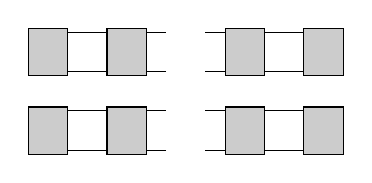
\begin{tikzpicture}
		\newcommand{\connectingRsAndSs}[1]
		{
			\draw[fill=black!20] (0,-.3) rectangle (0.5,.3) node[midway]{};
			\draw (0.5,-.25) rectangle (1,.25) node[midway]{};
			\draw[fill=black!20] (1,-.3) rectangle (1.5,.3) node[midway]{};
			\draw (1.75,-.25) --++ (-.25,0) --++(0,.5)--++(.25,0);
			\node at (2,0){\scriptsize};
			\draw (2.25,-.25) --++ (.25,0) --++(0,.5)--++(-.25,0);
			\draw[fill=black!20] (2.5,-.3) rectangle (3,.3) node[midway]{};
			\draw (3,-.25) rectangle (3.5,.25) node[midway]{};
			\draw[fill=black!20] (3.5,-.3) rectangle (4,.3) node[midway]{};
		}		
		
		\connectingRsAndSs{r}		
		\begin{scope}[yshift=-1cm]
			\connectingRsAndSs{s}
		\end{scope}
	\end{tikzpicture}
	\end{center}
	\caption{Satisfying }
	\label{fig:connectingRsAndSs}
\end{figure}

We are not quite done, however. We must show that we can replace the
{\em implicit} non-contact constraints that come with the use of
3-region variables by suitable -formulas.  For example, a
3-region variable  involves the implicit constraints
 and . Since the two conjuncts are identical in form,
we only show how to deal with .
Because the complement of  is  in general not connected, a direct 
use of  will result in a formula which is not satisfiable. 
Instead, we represent  as the sum of two regions  and 
with connected complements, and then proceed as before. In particular, we replace 
 by:

For ,  is a connected region that is disjoint from
. So,  is disjoint from  and , and hence 
disjoint from their sum . Fig~\ref{fig:crenellate} shows regions 
, for , which satisfy the above formula.
\begin{figure}[h]
	\begin{center}
	\scriptsize{
	\subfloat[The region  is the sum of  and .]{
		\begin{tikzpicture}
			\coordinate (P) at (0,0);
			\fill[black!25] (-1,1) rectangle (4.5,0);		
			\node at (-.5,.5) {};
			\fill[black!25] (-1,-1) rectangle (4.5,0);
			\node at (-.5,-.5) {};
			\draw (-1,0)--(4.5,0);
			\foreach \x in {0,1,2,3}
			{
				\ifnum \x=2					
				\else
					\draw[fill=white] () rectangle ();
					\draw[fill=gray!20] () rectangle () 
						node[midway]{};
				\fi
				\coordinate (P) at ();
			}
		\end{tikzpicture}
	}
	
	\subfloat[The mutually disjoint connected regions  and .]
	{
		\begin{tikzpicture}
			\coordinate (P) at (0,0);
			\fill[black!0] (-1,1) rectangle (4.5,0);
			\fill[black!25] (-1,-1) rectangle (4.5,0);
			\node at (-.5,-.5) {};
			\draw (-1,0)--(4.5,0);
			\foreach \x in {0,1,2,3}
			{
				\ifnum \x=2					
				\else
					\draw[fill=white] ()--() --() -- ();
					\draw[fill=gray!20] () rectangle ()
						node[midway]{};
				\fi
				\coordinate (P) at ();
			}			
			\fill[fill=gray!20] (.3,.2)--++(0,.4)--++(1.8,0)--++(0,-.3)--(1.5,.3)--++(0,-.1)--++(-.2,0)--++(0,.1)--(.5,.3)--++(0,-.1)--++(-.2,0)--++(0,.1);
			\draw (.3,.2)--++(0,.4)--++(1.8,0);
			\draw (2.1,.3)--(1.5,.3)--++(0,-.1)--++(-.2,0)--++(0,.1)--(.5,.3)--++(0,-.1)--++(-.2,0)--++(0,.1);		
			\draw[fill=gray!20,draw=black!95] (2.8,.6)--++(0.7,0)--++(0,-.4)--++(-.2,0)--++(0,.1)--(2.8,.3);
			\draw[draw=black!95] (2.5,.45) node {};
		\end{tikzpicture}
	}
	
	\subfloat[The mutually disjoint connected regions  and .]
	{
		\begin{tikzpicture}
			\coordinate (P) at (0,0);
			\fill[black!25] (-1,1) rectangle (4.5,0);		
			\node at (-.5,.5) {};
			\fill[black!0] (-1,-1) rectangle (4.5,0);			
			\draw (-1,0)--(4.5,0);
			\foreach \x in {0,1,2,3}
			{
				\ifnum \x=2					
				\else
					\draw[fill=white] ()--() --() -- ();
					\draw[fill=gray!20] () rectangle () 
						node[midway]{};
				\fi
				\coordinate (P) at ();
			}
			
			\fill[fill=gray!20] (.3,-.2)--++(0,-.4)--++(1.8,0)--++(0,.3)--(1.5,-.3)--++(0,.1)--++(-.2,0)--++(0,-.1)--(.5,-.3)--++(0,.1)--++(-.2,0)--++(0,-.1);
			\draw (.3,-.2)--++(0,-.4)--++(1.8,0);
			\draw (2.1,-.3)--(1.5,-.3)--++(0,.1)--++(-.2,0)--++(0,-.1)--(.5,-.3)--++(0,.1)--++(-.2,0)--++(0,-.1);		
			\draw[fill=gray!20,draw=black!95] (2.8,-.6)--++(0.7,0)--++(0,.4)--++(-.2,0)--++(0,-.1)--(2.8,-.3);
			\draw[draw=black!95] (2.5,-.45) node {};	
		\end{tikzpicture}
	}
	}
	\end{center}
	\caption{Eliminating the conjuncts of the form .} 
	\label{fig:crenellate}
\end{figure}
Let  be the result of replacing all the conjuncts (explicit
or implicit) containing the predicate , as just described. We have
thus shown that, if  is satisfiable over , then
 is positive, and that, if  is positive, then  is
satisfiable over . This completes the proof.

The final case we must deal with is that of . We use the
r.e.-hardness results already established for , and proceed,
as before, to eliminate occurrences of . Since all the polygons in 
the tuple satisfying  are quasi-bounded, we can eliminate 
all occurrences of  from  using 
Lemma~\ref{lma:Cci2BciStar}~(\emph{iii}). This completes the proof of 
Theorem~\ref{theo:undecidable}.




\section{ in 3D}\label{sec:Bci3D_C}

\newcommand{\ConRC}{{\sf ConRC}}


Denote by  the class of all connected topological spaces with regular closed regions. As shown in ~\cite{ijcai:kphz10}, every -formula satisfiable over  can be satisfied in a finite connected quasi-saw model and the problem  is \NP-complete.

\begin{theorem}
The problems , , coincide with , and so are all \NP-complete.
\end{theorem}
\begin{proof}
It suffices to show that every -formula  satisfiable over connected quasi-saws can also be satisfied over any of , for .
So suppose that  is satisfied in a model  based on a finite connected quasi-saw . Denote by  the set of points of depth  in , for .
Without loss of generality we may assume that there exists a point  with  for all . Indeed, if this is not the case, take the interpretation  obtained by extending  with such a point  and setting  iff  for some . Clearly, we have  iff , for any terms , . To see that  iff , recall that  is connected, and so  is disconnected in  iff there are two distinct points  connected by at least one path in  and such that no such path lies entirely in . It follows that if  is disconnected then , and so .  Thus, by adding  to  we cannot make a disconnected open set in  connected in .

We show now how  can be embedded into , for any .
First we take pairwise disjoint \emph{closed} balls  for all . We also select pairwise disjoint \emph{open} balls  for
, which are disjoint from all of the , and take  to be the complement of

(Note that  is connected for each ; all , for , are open, while  is closed).
We then expand every  to a set  in such a way that the following two properties are satisfied:
\begin{itemize}
\item[(A)] the , for , form a \emph{connected partition in } in the sense that  the  are regular closed sets in , whose interiors are non-empty, connected and  pairwise disjoint, and which sum up to the entire space;

\item[(B)] every point in , , is either

\begin{itemize}
\item[--]
in the interior of some  with , or

\item[--] on the boundary of \emph{all} of the  for which .
\end{itemize}
\end{itemize}
The required sets  are constructed as follows.
Let  be an enumeration of all the points in  with \emph{rational} coordinates.
For , we set  to be the closure of the infinite union , where the regular closed sets  are defined inductively as follows (see Fig.~\ref{fig:apollonian-app}):
\begin{itemize}
\item[--] Assuming that the  are already defined, let  be the first point in the list  such that , for all . Suppose  for . Take an open ball  of radius  centred in  and disjoint from the . For each  with , expand  by a closed ball in  and a closed rod connecting it to  in such a way that the ball and the rod are disjoint from the rest of the . The resulting set is denoted by .
\end{itemize}
\begin{figure}[h]
\begin{center}
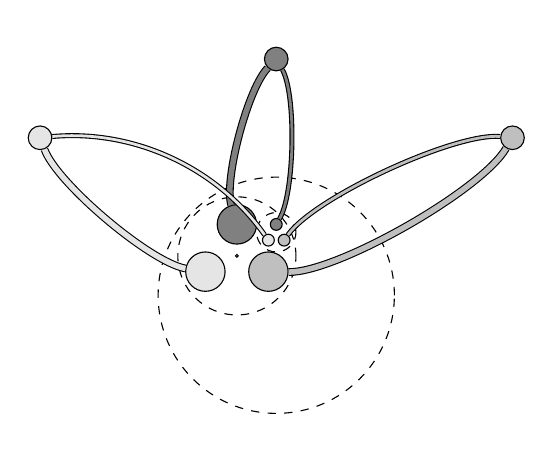
\begin{tikzpicture}[
clball/.style={circle,draw=black,minimum size=3mm,inner sep=0pt},
opball/.style={circle,dashed,draw=black,minimum size=30mm,inner sep=0pt}
]
\node [label=above:{\small }] (x1) at (0,-1)[clball,fill=Gray!20] {};
\node [label=above:{\small }] (x2) at (3,0)[clball,fill=Gray] {};
\node [label=above:{\small }] (x3) at (6,-1)[clball,fill=Gray!50] {};
\node [label=below:{\small }] (z1) at (3,-3)[opball] {};
\node [label=below:{\small }](c) at (2.5,-2.5)[opball,minimum size=15mm] {};
\node [label=below:{\small }](q) at (2.5,-2.5)[circle,inner sep=0pt,minimum size=1,draw=black] {};
\node (xc1) at (2.1,-2.7)[clball,fill=Gray!20,minimum size=5mm] {};
\node (xc2) at (2.5,-2.1)[clball,fill=Gray,minimum size=5mm] {};
\node (xc3) at (2.9,-2.7)[clball,fill=Gray!50,minimum size=5mm] {};
\draw[double=Gray!20,double distance=2pt] (xc1) to [bend left, looseness=0.5] (x1);
\draw[double=Gray,double distance=2pt] (xc2) to [bend left, looseness=0.5] (x2);
\draw[double=Gray!50,double distance=2pt] (xc3) to [bend right, looseness=0.5] (x3);
\node (cp) at (3,-2.2)[opball,minimum size=5mm] {};
\node (xcp1) at (2.9,-2.3)[clball,fill=Gray!20,minimum size=1.5mm] {};
\node (xcp2) at (3,-2.1)[clball,fill=Gray,minimum size=1.5mm] {};
\node (xcp3) at (3.1,-2.3)[clball,fill=Gray!50,minimum size=1.5mm] {};
\draw[double=Gray!20,double distance=1pt] (xcp1) to [bend right, looseness=0.9] (x1);
\draw[double=Gray,double distance=1pt] (xcp2) to [bend right, looseness=0.5] (x2);
\draw[double=Gray!50,double distance=1pt] (xcp3) to [bend left, looseness=0.5] (x3);
\end{tikzpicture}
\end{center}
\caption{The first two stages of filling  with , for , . (In , the sets  and  would not intersect.)}\label{fig:apollonian-app}
\end{figure}

Let  be the Boolean algebra of regular closed sets in  and let  be the Boolean algebra of regular closed sets in .
Define a map  from  to  by taking

By~(A),  is an isomorphic embedding of  into , that is,  preserves
the operations ,  and  and the constants  and .
Define an interpretation  over  by taking . To show that , it remains to prove that, for every ,  is connected if, and only if,  is connected. This equivalence follows from the fact that

where  is the set of all -successors of  of depth 0, which in turn is an immediate consequence of (B).
\end{proof}
\end{document}
